\documentclass[12pt,a4paper]{report}

% Packages
\usepackage{geometry}
\usepackage{amsmath}
\usepackage{amsfonts}
\usepackage{amssymb}
\usepackage{graphicx}
\usepackage{listings} % for code listing
\usepackage{subcaption}
\usepackage{tabularx}
\usepackage{hyperref}
\usepackage{wrapfig}

% Geometry
\geometry{a4paper, margin=1in}

% Title
\title{Computer Vision Homework Report \\ \Large Homework 4}

\author{Chinatip Lawansuk\\\\112998405}
\date{}


% For code listings
\lstset{
  basicstyle=\ttfamily\small,
  breaklines=true,
  frame=single,
  language=C++  % this line sets the language to C++
}

\begin{document}

\maketitle

\tableofcontents

\chapter{Introduction}
This project focuses on develop an algorithm to perform principle operations in Computer Vision from scratch.

\section{Objectives}
\begin{enumerate}
    \item Understand Theory of Computer Vision
    \item Improve C++/Python Programming Skill
\end{enumerate}

\section{Requirements}
\begin{enumerate}
    \item Write a Gaussian filter operation (customise parameters independently).
    \item Write a Sobel Edge Detection operation.
    \item Write a Active Contour (customise parameters independently).
\end{enumerate}

\section{System Configuration}
\subsection{Hardware}
\begin{itemize}
    \item CPU\@: Intel Core-i7
    \item GPU\@: NVIDIA
    \item RAM\@: 40 GB
\end{itemize}

\subsection{Software}
\begin{itemize}
    \item OS\@: Windows Subsystem Linux x64 (Ubuntu 22.04.3 LTS Kernel Ver. 5.15.90.1)
    \item GCC Version\@: \verb|11.4.0 x86_64-linux-gnu|
    \item OpenCV Version\@: \verb|4.5.4+dfsg-9ubuntu4|
\end{itemize}

\chapter{Solution, Explanation, and Result}
In this project, code explanation is embedded in the comment section in the code.

\section{Main Function}
The main function of the program will load the desired picture, apply the function sequentially, display on the window, and write a new file for the proceeded image and video. This main function also control the iteration for Active Contour algorithm.
\begin{lstlisting}
#include <stdio.h>
#include <opencv2/opencv.hpp>
#include <unistd.h>
#include <string.h>
#include "include/func.hpp"
#include <opencv2/videoio/videoio_c.h>

#define MAX_LEN 250

// path for lab
#define BASE_PATH "/home/chinatip/computer-vision-lab-fall-2023/homework4"
#define SRC_PATH "test_img"
#define OUT_PATH "output"

// define file name, can uncomment to select the input
#define FILENAME "img1"
// #define FILENAME "img2"
// #define FILENAME "img3"

#define EXT "jpg"

Mat canvas;

void appendImgToCanvas(Mat);

int main(int argc, char **argv)
{

    Mat og_img;
    char og_file[MAX_LEN] = "", out_file[MAX_LEN] = "";
    snprintf(og_file, MAX_LEN, "%s/%s/%s.%s", BASE_PATH, SRC_PATH, FILENAME, EXT);

    og_img = imread(og_file);

    if (!og_img.data)
    {
        printf("No image data \n");
        return -1;
    }
    else
    {
        printf("Original Img Size: w x h %d x %d\n", og_img.cols, og_img.rows);
    }

    appendImgToCanvas(og_img);
    Mat bw_img;
    bw_img = applyGreyscaleFilter(og_img);

    Mat res_img, selected_img;

    Mat gaussian_filter = createGaussianFilter(3, 1);
    res_img = applyFilter(bw_img, gaussian_filter, 1, false);
    printf("Gaussian Filter Img Size: w x h %d x %d\n", res_img.cols, res_img.rows);

    appendImgToCanvas(res_img);

    Mat sobelx;
    sobelx = applySobelX(res_img);
    appendImgToCanvas(sobelx);

    Mat sobely;
    sobely = applySobelY(res_img);
    appendImgToCanvas(sobely);

    Mat magnitude;
    magnitude = calculateEdgeStrength(sobelx, sobely);

    Mat direction;
    direction = calculateEdgeDirection(sobelx, sobely);

    Mat output;
    magnitude.copyTo(output);
    showGradient(output, magnitude, direction, 3);
    snprintf(out_file, MAX_LEN, "%s/%s/first_order_gvf.jpg", BASE_PATH, OUT_PATH);
    imwrite(out_file, output);

    Mat mag2, dir2, dx, dy, res;
    dx = applySobelX(magnitude);
    dy = applySobelY(magnitude);
    mag2 = calculateEdgeStrength(dx, dy);
    dir2 = calculateEdgeDirection(dx, dy);

    mag2.copyTo(output);
    showGradient(output, mag2, dir2, 3);
    snprintf(out_file, MAX_LEN, "%s/%s/second_order_gvf.jpg", BASE_PATH, OUT_PATH);
    imwrite(out_file, output);

    vector<ContourPoint> contour;

    VideoWriter video;
    char video_name[100] = "\0";
    snprintf(video_name, 99, "%s/%s/vid_%s.mp4", BASE_PATH, OUT_PATH, FILENAME);
    video.open(video_name, CV_FOURCC('m', 'p', '4', 'v'), 10, og_img.size(), true);

    // We apply termination logic outside the active contour function
    // it is done by calculate energy over 4 last epochs
    // if it oscillates or stable, we increase count by 1
    // The threshold of count is 20 to help avoid local minima

    contour = initContourPointCircle(magnitude.cols / 2, magnitude.rows / 2, 400, 200);
    float alpha = 0.05, beta = 0.00001, gamma = 0.5;
    float min_e = numeric_limits<float>::max(), current_e, e_1 = 0, e_2 = 0, e_3 = 0, e_4 = 0, diff1, diff2, diff3;
    bool isOscillating = false, isConverging = false;
    int osc_cnt = 0;
    vector<Mat> buf;
    char iter_text[25] = "\0";
    for (int k = 0; k < 10000; k++)
    {
        Mat i;
        activeContour(mag2, dir2, contour, alpha, beta, gamma);
        current_e = contourEnergy(contour);

        Mat mag_with_field;
        og_img.copyTo(mag_with_field);
        i = showSnake(mag_with_field, contour);

        // calculate energy over 4 latest energy to check
        // if converge or oscillate
        e_4 = e_3;
        e_3 = e_2;
        e_2 = e_1;
        e_1 = current_e;
        diff1 = e_2 - e_1;
        diff2 = e_3 - e_2;
        diff3 = e_4 - e_3;
        isOscillating = (diff1 * diff2 < 0) && (diff2 * diff3 < 0);
        isConverging = std::abs(diff1) == std::abs(diff2) && std::abs(diff2) == std::abs(diff3);

        if (!(isOscillating && isConverging))
        {
            min_e = current_e;
            osc_cnt = 0;
        }
        else
        {
            osc_cnt += 1;
            // termination condition
            if (osc_cnt == 20)
            {

                snprintf(iter_text, 24, "Iteration: %d", k);
                putText(i, iter_text, Point2i(10, 30), FONT_HERSHEY_SIMPLEX, 1, (0, 0, 0), 2);
                printf("Frame %d %f\n", k, min_e);
                snprintf(out_file, MAX_LEN, "%s/%s/result_%s.%s", BASE_PATH, OUT_PATH, FILENAME, EXT);
                imwrite(out_file, i);
                imshow("Original", i);
                video.write(i);
                video.release();
                waitKey(10);
                break;
            }
        }

        if (k % 10 == 0)
        {
            snprintf(iter_text, 24, "Iteration: %d", k);
            putText(i, iter_text, Point2i(10, 30), FONT_HERSHEY_SIMPLEX, 1, (0, 0, 0), 2);
            imshow("Original", i);
            video.write(i);
            waitKey(10);
        }
    }
    printf("Finish\n");
    waitKey(0);
    return 0;
}

void appendImgToCanvas(Mat img)
{
    if (canvas.empty())
    {
        canvas = img;
    }
    else
    {
        Size s(canvas.cols + img.cols + 5, canvas.rows > img.rows ? canvas.rows : img.rows);
        size_t old_w = canvas.cols;
        copyMakeBorder(canvas, canvas, 0, 0, 0, img.cols + 5, BORDER_CONSTANT, Scalar(0, 0, 0, 0));
        img.copyTo(canvas(Rect(old_w + 5, 0, img.cols, img.rows)));
    }
}
\end{lstlisting}
\begin{figure}[!htb]
    \centering
    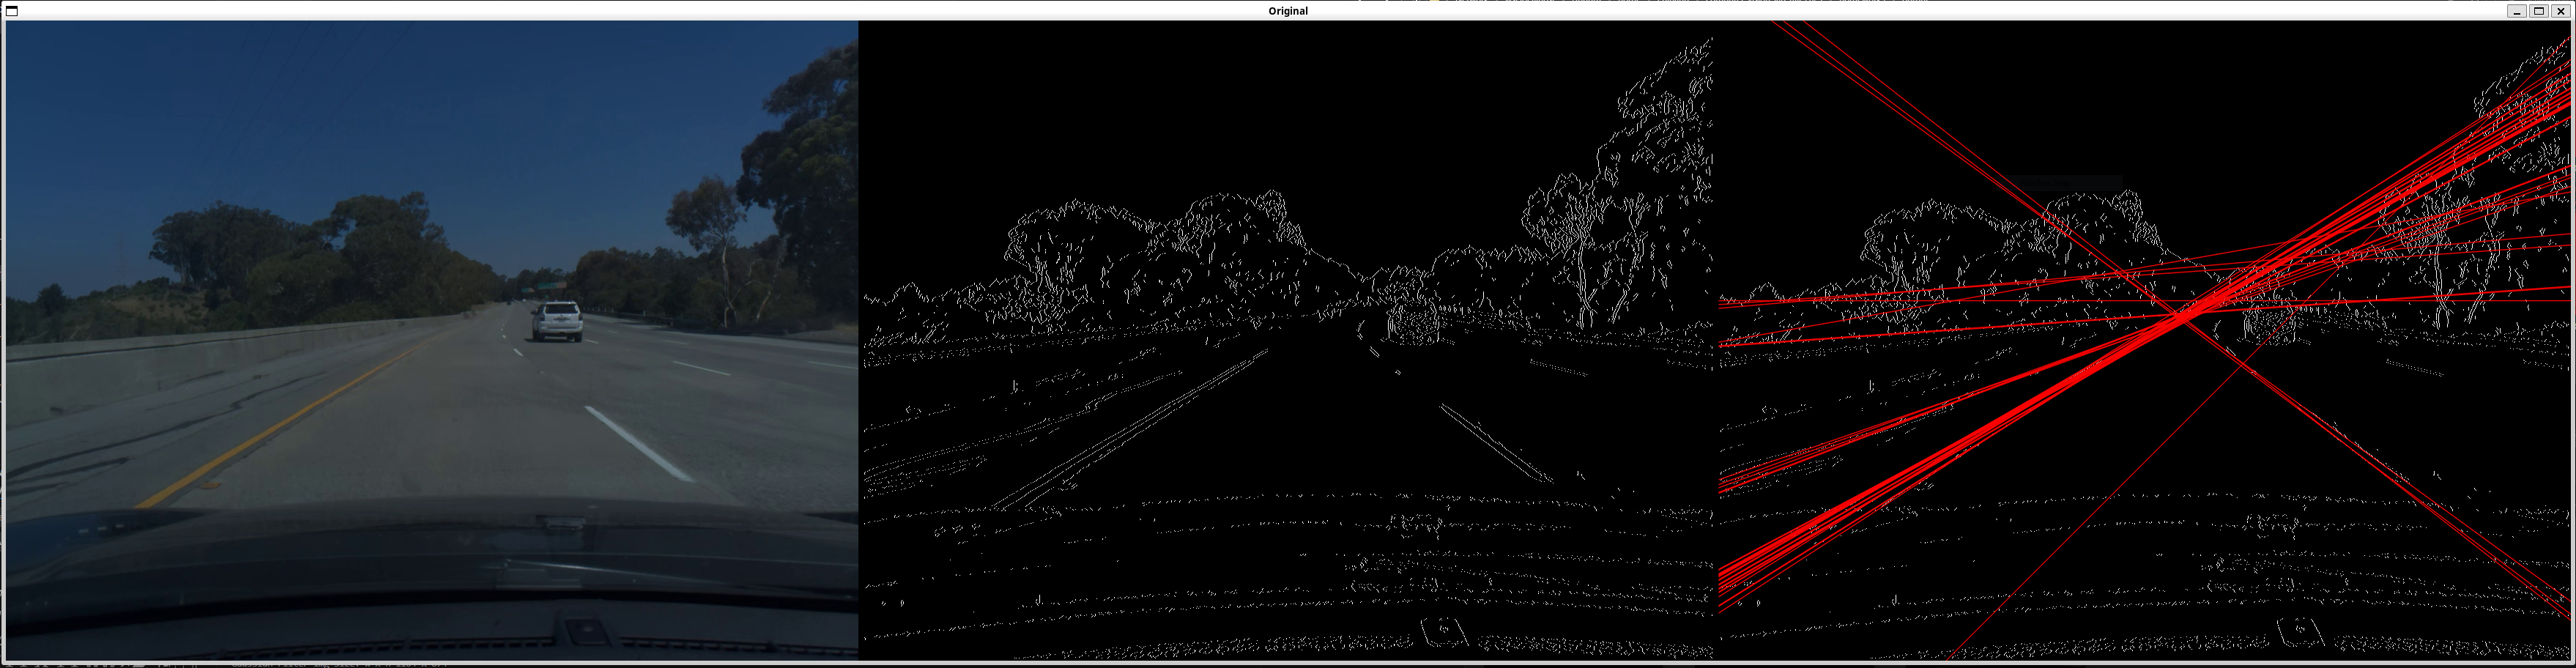
\includegraphics[width=1\linewidth]{program.png}
    \caption{Program Output (Automatic place image in frame)}
\end{figure}
\clearpage


\section{Applying Greyscale Filter}
\begin{tabular}{lll}
    Input  & : & Matrix of Input Image  \\
    Output & : & Matrix of Output Image \\
\end{tabular}
\begin{lstlisting}
Mat applyGreyscaleFilter(Mat img)
{
    // Create New Image as Output Image
    Mat bw_img(img.size(), img.type());
    for (int j = 0; j < img.rows; j++)
    {
        for (int i = 0; i < img.cols; i++)
        {
            // Get the pixel value from the original image
            Vec3b brg_px = img.at<Vec3b>(j, i);

            // Normal average function ie. sum(xn)/n ;
            int b = (brg_px[0] + brg_px[1] + brg_px[2]) / 3;

            // Write back to every channel
            brg_px[0] = b;
            brg_px[1] = b;
            brg_px[2] = b;

            // Write to new image buffer
            bw_img.at<Vec3b>(j, i) = brg_px;
        }
    }
    // return the output image
    return bw_img;
}
\end{lstlisting}
\begin{figure}[!htb]
    \centering
      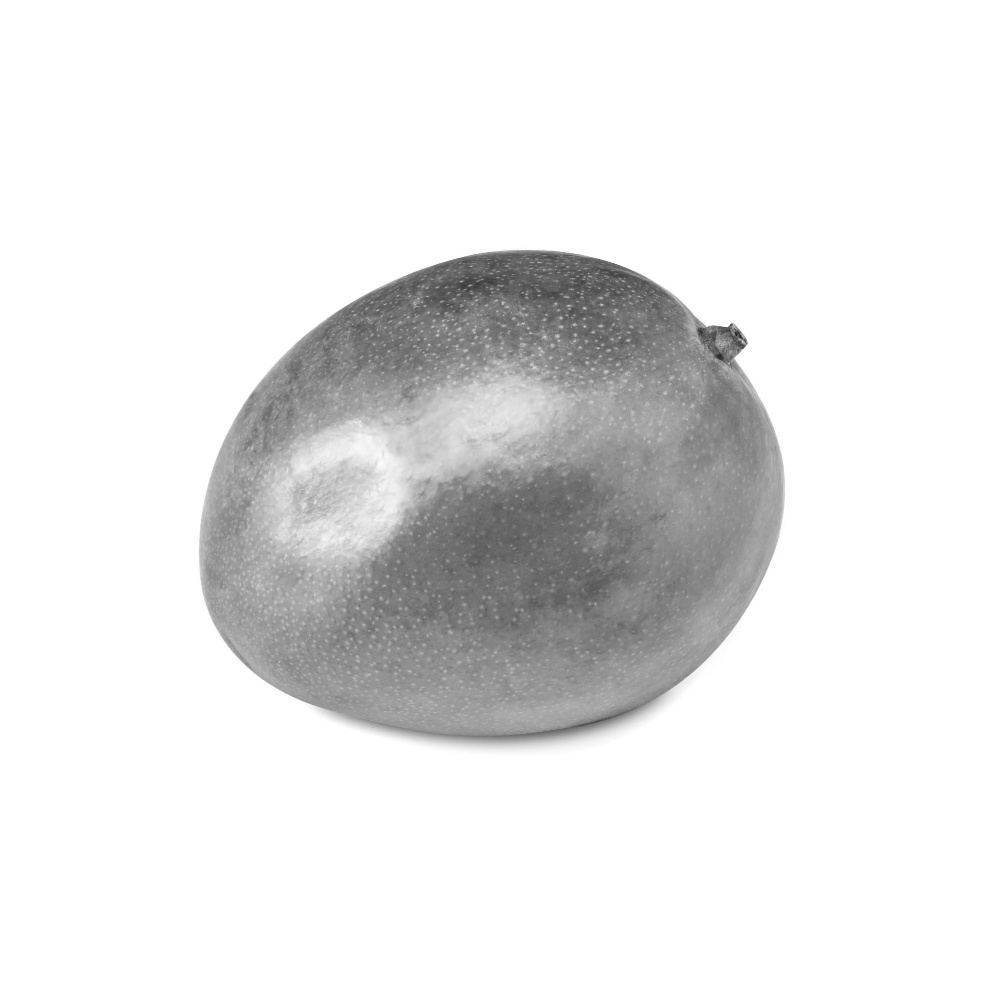
\includegraphics[height=0.4\paperheight]{output/grey_scale.jpg}
    \caption{Output of Grey Scale function}
\end{figure}
\clearpage

\section{Apply Gaussian Filter}
Since using filter can be reused in multiple step, the general function is extracted below.
In order to use Gaussian filter, we need to create kernel using provided function below, then applt with the general function.
\subsection{Create Gaussian Filter}
\begin{tabular}{lll}
    Input  & : & Kernel size (Integer)     \\
           &   & Sigma (float)             \\
    Output & : & Matrix of Gaussian Filter \\
\end{tabular}
\begin{lstlisting}
float calculateGaussian(int x, int y, float sigma)
{
    return (1 / (CV_2PI * sigma * sigma)) * (powf32(K_E, -1 * ((x * x) + (y * y)) / (2 * sigma * sigma)));
}

Mat createGaussianFilter(int size, float sigma)
{
    int center = size / 2;
    Mat kernel = Mat::zeros(size, size, CV_32F);
    for (int j = 0; j < kernel.rows; j++)
    {
        for (int i = 0; i < kernel.cols; i++)
        {
            kernel.at<float>(j, i) = calculateGaussian(i - center, j - center, sigma);
        }
    }
    return kernel;
}
\end{lstlisting}

\subsection{Apply Filter}
\begin{tabular}{lll}
    Input  & : & Matrix of Input Image  \\
           &   & Kernel Matrix          \\
           &   & Stride size (Integer)  \\
           &   & Suppress Border (Bool) \\
    Output & : & Matrix of Output Image \\
\end{tabular}
\begin{lstlisting}
Mat applyFilter(Mat img, Mat kernel, int stride, bool suppress_border)
{

    // calculate kernel offset ie. number of pixel before and
    // after since the target pixel will be the center of
    // matrix,
    // in order to get the neighbour pixel with size of kernel
    // size, offset will be applied for both before, and after
    // the target pixel
    // example
    // width = 5 => offset = (int)5/2 = 2;
    // px   ... k   n-offset    ... n   ... n+offset    k
    int ker_x_offset = kernel.cols / 2;
    int ker_y_offset = kernel.rows / 2;

    int padding = ker_x_offset;

    // get kernel size
    int ker_w = kernel.cols;
    int ker_h = kernel.rows;

    // calculate output image size
    int out_w = ((img.cols + (2 * padding) - kernel.cols) / stride) + 1;
    int out_h = ((img.rows + (2 * padding) - kernel.rows) / stride) + 1;

    // create intermediate buffer and add padding, size is
    // w+(2*padding),h+(2*padding) then copy the content
    // of image to the buffer
    Mat padded;
    padded = Mat::zeros(img.rows + (2 * padding), img.cols + (2 * padding), CV_32SC3);
    int dtype = img.type();

    // here, we convert data type while copy to make it compatible
    // for higher precision computation
    // check if input is uint8 or int 32
    // if uint8 then we will channel-wise copy to padded buffer
    // due to different data alignment
    // if int38 then we will pixel-wise copy to padded buffer
    switch (dtype)
    {
    case CV_32SC3:
        for (int j = 0; j < img.rows; j++)
        {
            for (int i = 0; i < img.cols; i++)
            {
                padded.at<Vec3i>(j + padding, i + padding) = img.at<Vec3i>(j, i);
            }
        }
        break;
    case CV_8UC3:
        for (int j = 0; j < img.rows; j++)
        {
            for (int i = 0; i < img.cols; i++)
            {
                for (int k = 0; k < 3; k++)
                {
                    padded.at<Vec3i>(j + padding, i + padding)[k] = img.at<Vec3b>(j, i)[k];
                }
            }
        }
        break;
    default:
        break;
    }

    // create output buffer with calculated output size
    // data type need to be vector of signed int 32 bit
    // in case negative data is possible, this can help
    // preserve information through the convolution process
    // and rasterise to 8 bit at the last step
    Mat img_res = Mat::zeros(out_h, out_w, CV_32SC3);

    Vec3i res(0, 0, 0);

    // iterate over the size of input image
    for (int img_j = 0; img_j < img.rows; img_j += stride)
    {
        for (int img_i = 0; img_i < img.cols; img_i += stride)
        {
            // check if it is a border and suppress border
            // if selected
            if (img_i < ker_w || img_j < ker_h || img_i > img.cols - ker_h - 1 || img_j > img.rows - ker_h - 1)
            {
                if (suppress_border)
                {
                    res = Vec3i(0, 0, 0);
                    img_res.at<Vec3i>((img_j) / stride, (img_i) / stride) = res;
                    continue;
                }
            }

            // get windowed matrix from the padded buffer with
            // the size of kernel size, and target pixel is in
            // the center of windowed matrix
            Mat windowed = padded(Rect(img_i, img_j, ker_w, ker_h));
            res = Vec3i(0, 0, 0);
            float tmp = 0;
            float tmp1 = 0;
            float tmp2 = 0;
            float tmp3 = 0;

            // item-wise multiply windowed matrix with kernel
            // matrix and summarise
            for (int ker_j = 0; ker_j < kernel.rows; ker_j++)
            {
                for (int ker_i = 0; ker_i < kernel.cols; ker_i++)
                {
                    Vec3b t = windowed.at<Vec3i>(ker_j, ker_i);
                    float k = kernel.at<float>(ker_j, ker_i);
                    tmp += (t[0] * k);
                    tmp1 += (t[0] * k);
                    tmp2 += (t[1] * k);
                    tmp3 += (t[2] * k);
                }
            }
            res[0] = tmp1;
            res[1] = tmp2;
            res[2] = tmp3;

            // write to output buffer
            img_res.at<Vec3i>((img_j) / stride, (img_i) / stride) = res;
        }
    }
    // return the output image
    return img_res;
}
\end{lstlisting}
\begin{figure}[!htb]
    \centering
    %   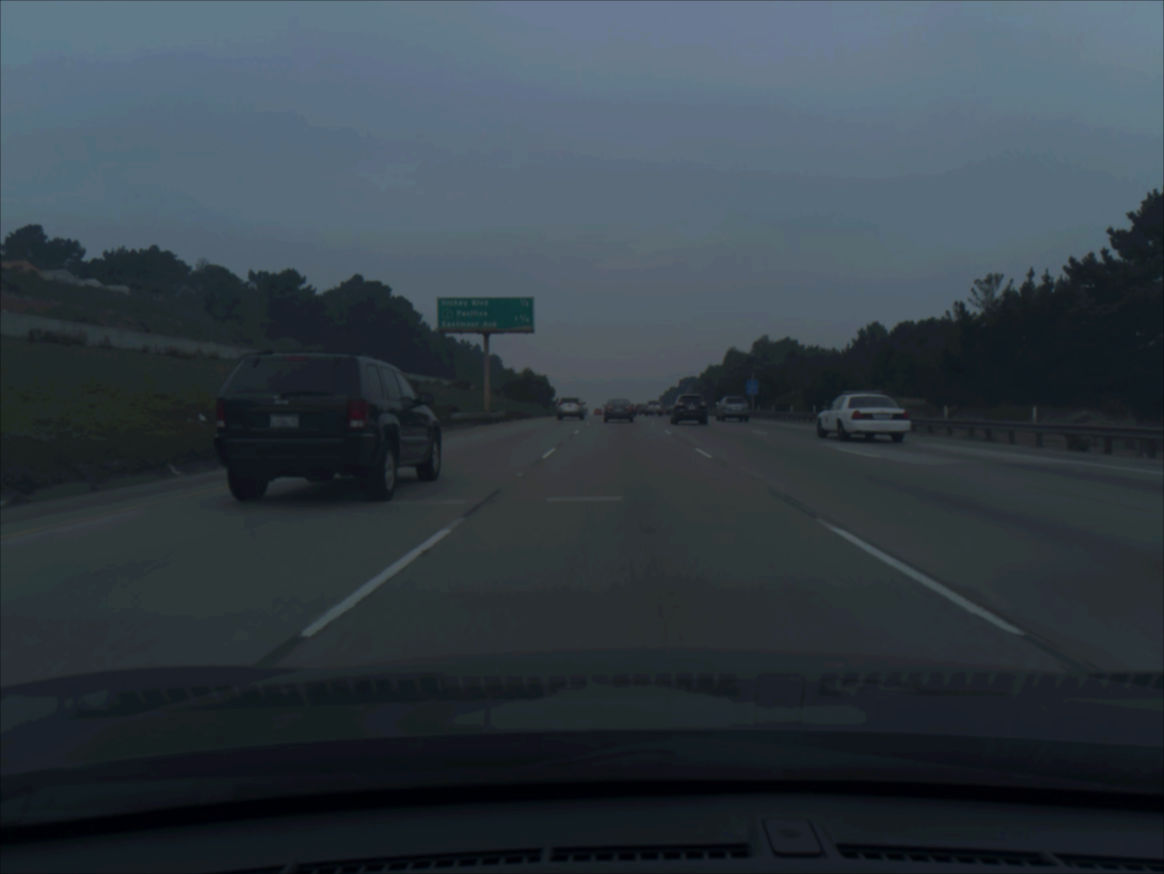
\includegraphics[height=0.4\paperheight]{output/img2_q1_K3_SIG_1.0.png}
      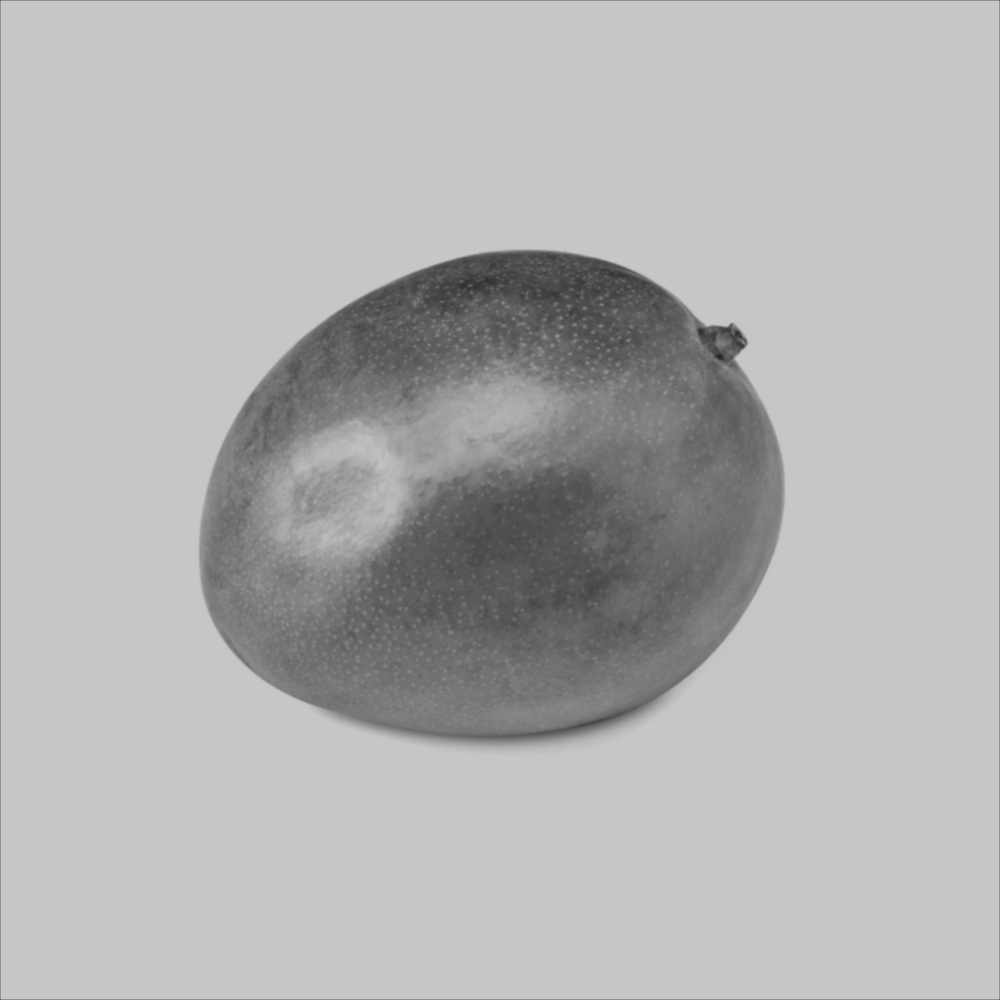
\includegraphics[height=0.4\paperheight]{output/gaussian.jpg}
    \caption{Output of Gaussian Filter function}
\end{figure}
\clearpage


\section{Apply Edge Detector and Related Functions}
\subsection{Sobel X and Y}
This only apply Sobel kernel.
\begin{tabular}{lll}
    Input  & : & Matrix of Input Image  \\
    Output & : & Matrix of Output Image \\
\end{tabular}
\begin{lstlisting}
Mat applySobelX(Mat img_in)
{
    float c_sobelX[] = {-1, 0, 1,
                        -2, 0, 2,
                        -1, 0, 1};
    Mat sobelX(3, 3, CV_32F, c_sobelX);
    Mat result = applyFilter(img_in, sobelX, 1, true);
    return result;
}

Mat applySobelY(Mat img_in)
{
    float c_sobelY[] = {-1, -2, -1,
                          0,  0,  0,
                          1,  2,  1};
    Mat sobelY(3, 3, CV_32F, c_sobelY);
    Mat result = applyFilter(img_in, sobelY, 1, true);
    return result;
}
\end{lstlisting}
\begin{figure}[!htb]
    \centering
      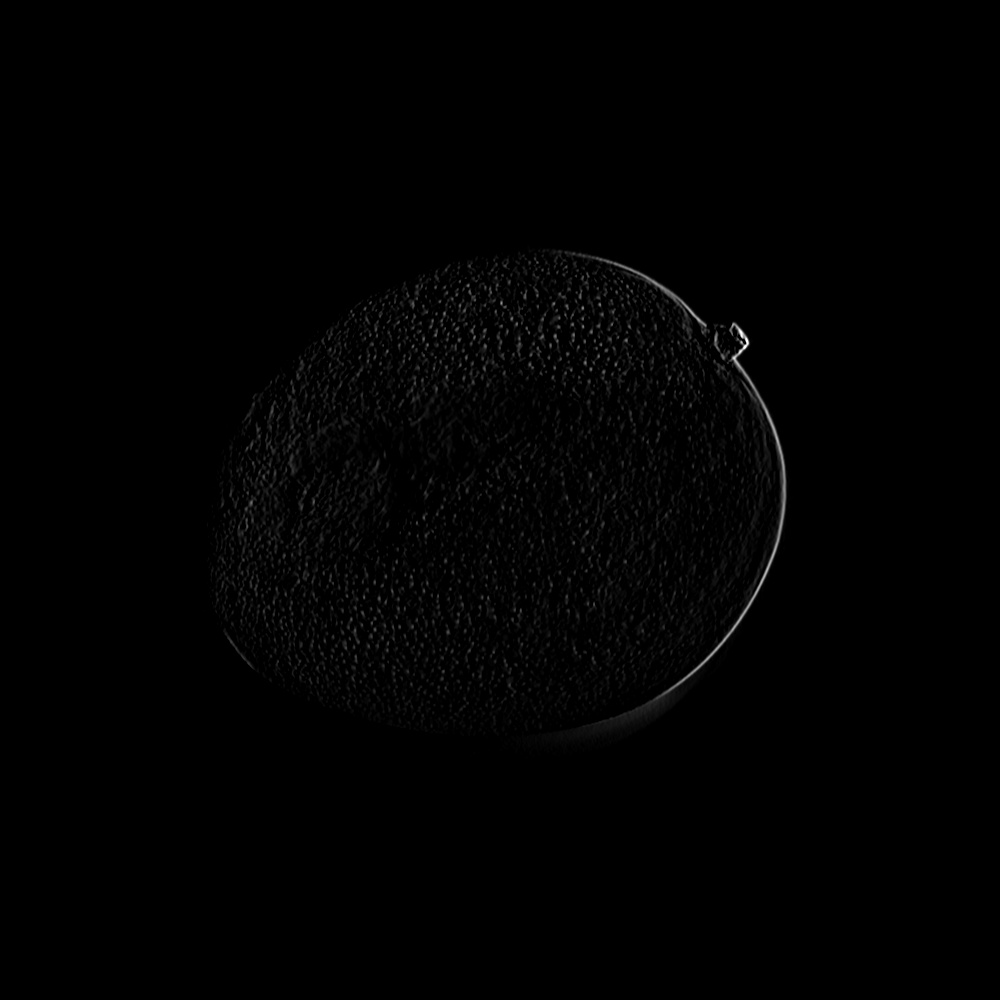
\includegraphics[height=0.4\paperheight]{output/sobel_x.jpg}
      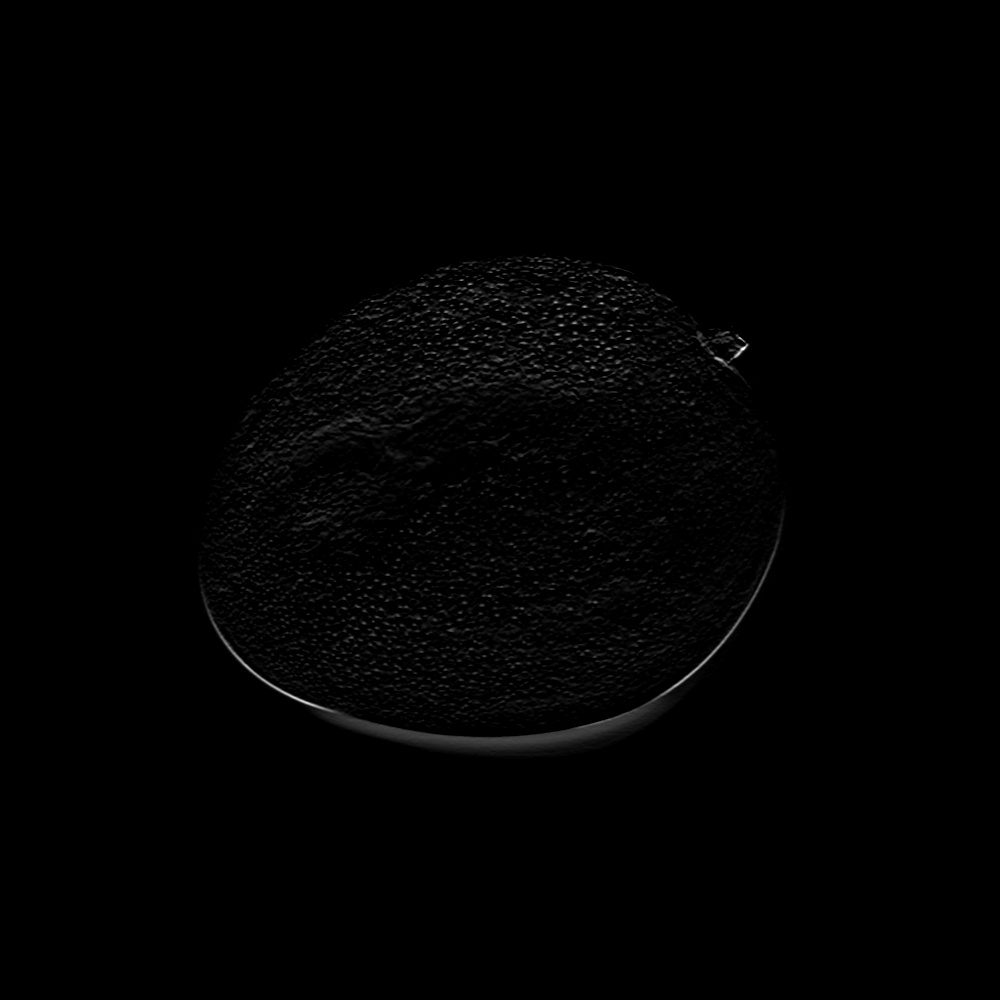
\includegraphics[height=0.4\paperheight]{output/sobel_y.jpg}
    \caption{Output of Sobel X (Upper) and Sobel Y (Lower)}
\end{figure}
\clearpage


\subsection{Gradient Calculation}
This step, we will get edge strength and direction.

\subsubsection{Edge Strength}
\begin{tabular}{lll}
    Input  & : & Matrix of Input Sobel X \\
           & : & Matrix of Input Sobel Y \\
    Output & : & Matrix of Edge Strength \\
\end{tabular}
\begin{lstlisting}
Mat calculateEdgeStrength(Mat x, Mat y)
{
    Mat strength = Mat::zeros(x.rows, x.cols, CV_32FC3);
    float tmp = 0;
    for (int j = 0; j < strength.rows; j += 1)
    {
        for (int i = 0; i < strength.cols; i += 1)
        {
            for (int k = 0; k < 3; k++)
            {
                // Strength of pixel is calculated by
                // sqrt(gx^2 + gy^2)
                tmp = (x.at<Vec3i>(j, i)[k] * x.at<Vec3i>(j, i)[k]) + (y.at<Vec3i>(j, i)[k] * y.at<Vec3i>(j, i)[k]);
                strength.at<Vec3f>(j, i)[k] = sqrtf32(tmp);
            }
        }
    }

    return strength;
}
\end{lstlisting}
\begin{figure}[!htb]
    \centering
      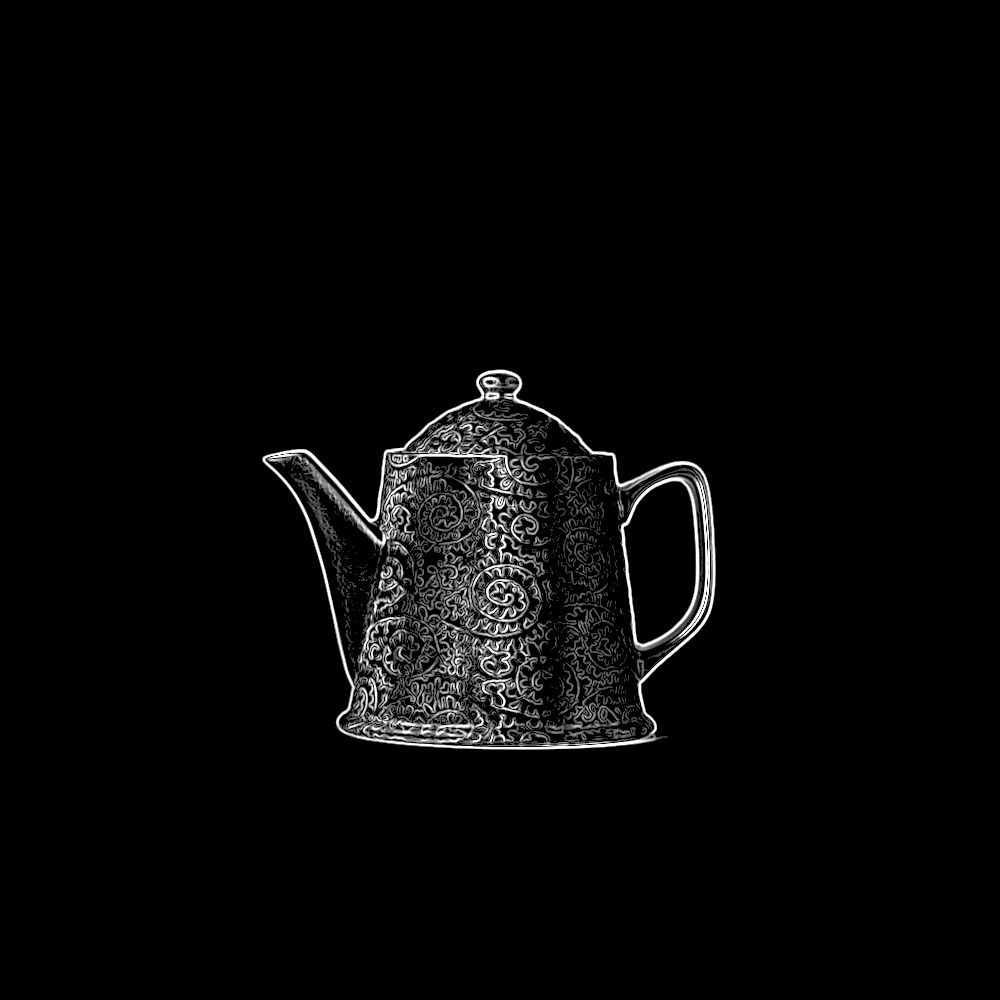
\includegraphics[height=0.4\paperheight]{output/magnitude.jpg}
    \caption{Edge Strength}
\end{figure}
\clearpage

\subsubsection{Edge Direction}
\begin{tabular}{lll}
    Input  & : & Matrix of Input Sobel X  \\
           & : & Matrix of Input Sobel Y  \\
    Output & : & Matrix of Edge Direction \\
\end{tabular}
\begin{lstlisting}
Mat calculateEdgeDirection(Mat x, Mat y)
{
    Mat direction = Mat::zeros(x.rows, x.cols, CV_32FC3);
    for (int j = 0; j < direction.rows; j += 1)
    {
        for (int i = 0; i < direction.cols; i += 1)
        {
            for (int k = 0; k < 3; k++)
            {
                // direction of pixel is calculated by
                // atan(y/x)
                direction.at<Vec3f>(j, i)[k] = atan2f32(y.at<Vec3f>(j, i)[k], x.at<Vec3f>(j, i)[k]) * 10;
            }
        }
    }
    return direction;
}
\end{lstlisting}
\begin{figure}[!htb]
    \centering
      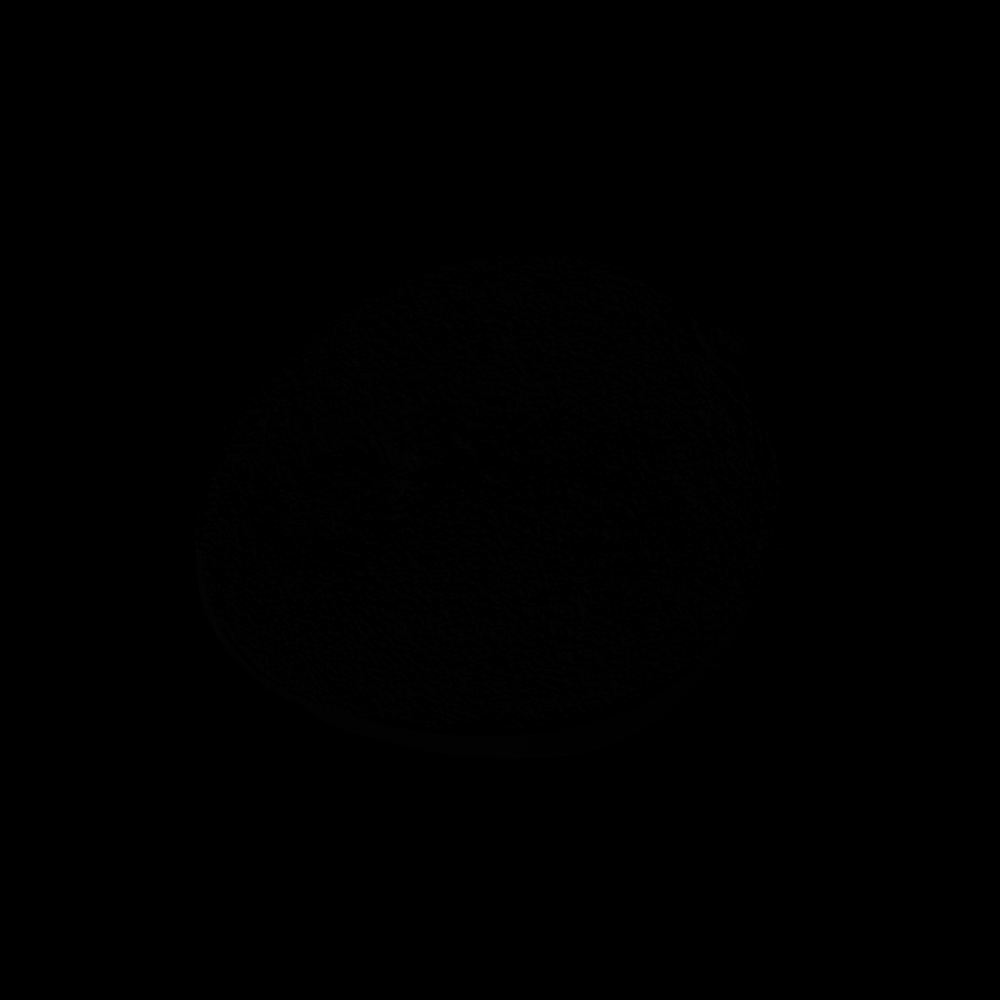
\includegraphics[height=0.4\paperheight]{output/direction.jpg}
    \caption{Direction of Gradient}
\end{figure}
\clearpage

\subsection{Active Contour}

\subsubsection{\(ContourPoint\) Data Type}
This inherit from \(cv2::Point2f\) class with additional property named \(energy\) used to store energy of each point.
\begin{lstlisting}
/**
* @brief Class representing a point with additional energy attribute.
*
* Inherits from OpenCV's Point2f class and adds an energy attribute.
* This can be used to represent points in an image with an associated energy value.
*/
class ContourPoint : public Point2f
{
public:
    float energy; ///< Energy value of the contour point.
};
\end{lstlisting}


\subsubsection{Initialise Contour}
This function will intialise Contour points in a circle shape.\\
\begin{tabular}{lll}
    Input  & : & center of contour x (int)  \\
           & : & center of contour y (int) \\
           & : & radius of contour (int) \\
           & : & number of point (int) \\
\end{tabular}
\begin{lstlisting}
/**
* @brief Initialise contour points in a circular pattern.
*
* This function creates a set of contour points arranged in the shape of a circle.
* It is useful for initializing contour-based algorithms, especially for circular objects.
*
* @param cx The x-coordinate of the circle's center.
* @param cy The y-coordinate of the circle's center.
* @param r The radius of the circle.
* @param quantity The number of contour points to generate.
* @return vector<ContourPoint> A vector of contour points arranged in a circular pattern.
*/
vector<ContourPoint> initContourPointCircle(int cx, int cy, int r, int quantity)
{
    vector<ContourPoint> tmp;
    float theta = 0, d_theta = (2 * CV_PI) / quantity;

    for (int i = 0; i < quantity; i++)
    {
        float x, y;
        // Calculate the x and y coordinates using polar to
        // Cartesian conversion
        x = (r * cosf32(theta)) + cx;
        y = (r * sinf32(theta)) + cy;

        // Create a ContourPoint and set its properties
        ContourPoint p;
        p.x = x;
        p.y = y;

        // Since we try to minimise the energy, we initialise
        // the energy to the maximum float value
        p.energy = numeric_limits<float>::max();

        // Add the ContourPoint to the vector
        tmp.push_back(p);
        theta += d_theta;
    }

    // Return the vector of contour points
    return tmp;
}
\end{lstlisting}




\subsubsection{Active Contour}
This function will perform Active Contour, by searching around each contour points and selecting the point that gives minimum energy to be a new contour point. While iteratively execute this function, the contour will converge to the minimum total energy.
The energy function is given by
\[E_{total}= \alpha E_{cont} + \beta E_{curv} + \gamma E_{grad}\]\\
\[E_{cont} = ||p-pp||^2\]\\
\[E_{curv} = ||pp+pn-2p||^2\]\\
\[E_{grad} = -||\nabla I(p)||\]\\
which \(p\) is current contour point, \(pn\) is next contour point , and \(pp\) is previous contour point.

\begin{tabular}{lll}
    Input  & : & Matrix of Input Edge Strength  \\
           & : & Matrix of Input Edge Direction \\
           & : & List of Contour Point (std::vector\(\langle ContourPoint\rangle\)) \\
           & : & alpha (float)\\
           & : & beta (float)\\
           & : & gamma (float)\\
\end{tabular}
\begin{lstlisting}
/**
* @brief Perform the active contour (snake) algorithm on an image.
*
* This function iteratively adjusts the positions of contour points to align with image features
* like edges, based on an energy minimization process. The energy terms include continuity,
* curvature, and image forces.
*
* @param magnitude The magnitude of the gradient of the image.
* @param direction The direction of the gradient of the image.
* @param contour A reference to a vector of ContourPoint representing the initial contour.
* @param alpha The weight for the continuity energy term.
* @param beta The weight for the curvature energy term.
* @param gamma The weight for the image energy term.
*/
void activeContour(Mat magnitude, Mat direction, vector<ContourPoint> &contour, float alpha, float beta, float gamma)
{
    int p_cnt = contour.size();
    vector<ContourPoint> prev_contour(contour);

    for (int i = 0; i < p_cnt; i++)
    {
        // Retrieve previous, current, and next points in the contour
        ContourPoint pp, p, pn;
        pp = prev_contour[(i - 1 + p_cnt) % p_cnt];
        p = prev_contour[i % p_cnt];
        pn = prev_contour[(i + 1) % p_cnt];

        // Energy terms
        float e_cont, e_curve, e_image, e_point;

        // Search window settings
        int s_size = 25, s_offset = s_size / 2;
        int min_i = 0, min_j = 0;
        float min_e_point = numeric_limits<float>::max();

        // Search within the window to minimise energy
        for (int wj = 0; wj < s_size; wj++)
        {
            for (int wi = 0; wi < s_size; wi++)
            {
                ContourPoint tmp;

                // Candidate point within the window
                tmp.x = p.x - s_offset + wi;
                tmp.y = p.y - s_offset + wj;
                int tmp_mag = magnitude.at<Vec3b>((int)tmp.y, (int)tmp.x)[0];

                // Calculate energy terms
                e_cont = powf32((pn + pp - 2 * tmp).x, 2) + powf32((pn + pp - 2 * tmp).y, 2);
                e_curve = powf32((tmp - pp).x, 2) + powf32((tmp - pp).y, 2);
                e_image = -tmp_mag * tmp_mag;
                e_point = (alpha * e_cont) + (beta * e_curve) + (gamma * e_image);

                // Update if a lower energy point is found
                if (e_point < min_e_point)
                {
                    min_e_point = e_point;
                    min_i = tmp.x;
                    min_j = tmp.y;
                }
            }
        }

        // Update the contour point with the minimum energy point found
        contour[i].x = min_i;
        contour[i].y = min_j;
        contour[i].energy = min_e_point;
    }
}
\end{lstlisting}
\begin{figure}[!htb]
    \centering
      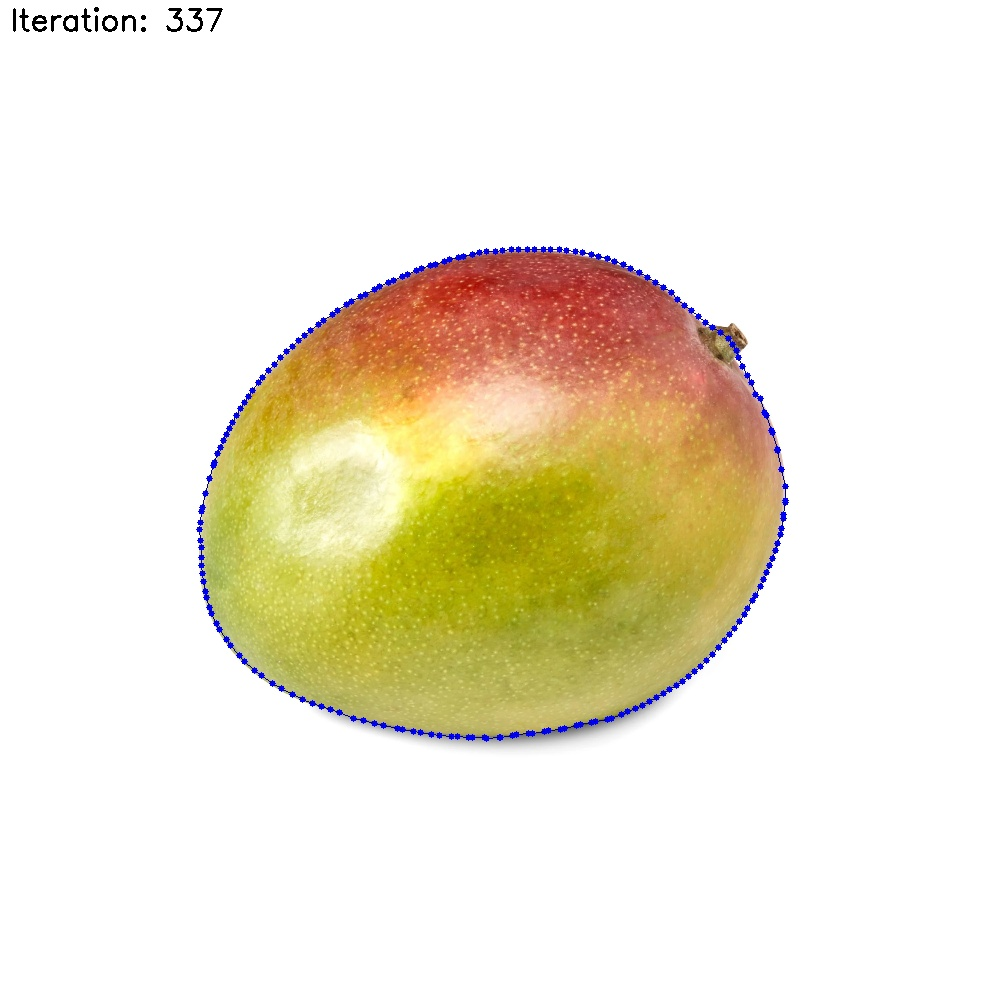
\includegraphics[height=0.4\paperheight]{output/result_img1.jpg}
    \caption{Contour points calculated from the function (with snake, embedded in picture)}
\end{figure}
\clearpage

\subsubsection{Contour Energy Calculation}
\begin{tabular}{lll}
    Input  & : & List of Contour Point (std::vector\(\langle ContourPoint\rangle\))  \\
    Output & : & total contour energy (float)   \\
\end{tabular}
\begin{lstlisting}
/**
* @brief Calculate the total energy of a contour.
*
* This function computes the sum of the energy values of each point in the contour.
* It is useful for evaluating the overall energy of the contour, which can be a measure of its
* alignment with image features or its smoothness, depending on the energy model used.
*
* @param contour A reference to a vector of ContourPoint, each with an associated energy value.
* @return float The total energy of the contour.
*/
float contourEnergy(vector<ContourPoint> &contour)
{
    float tmp = 0;
    int cnt = contour.size();

    // Iterate over each point in the contour
    for (int c = 0; c < cnt; c++)
    {
        // Check if the energy is not infinity and not the
        // maximum float value
        // This is done to ensure that only valid, finite
        // energy values are summed
        if (!isinff(contour[c].energy) && contour[c].energy != numeric_limits<float>::max())
        {
            // Add the point's energy to the total
            tmp += contour[c].energy;
        }
    }

    return tmp; // Return the total energy of the contour
}
\end{lstlisting}

\subsubsection{Iteration and Termination Logic}
This section performed in main function of the program it controls the iteration process by observing 4 latest previous contour energy. If it converge to a single value or oscillate, it is considered as a stable state and terminate iteration. To ensure the oscillation is a true oscillation in global minumum region, not the local minumum region, we also apply counting. It is considered as a global minumum when 20 consequent occurred.
\begin{lstlisting}
    // We apply termination logic outside the active contour function
    // it is done by calculate energy over 4 last epochs
    // if it oscillates or stable, we increase count by 1
    // The threshold of count is 20 to help avoid local minima

    contour = initContourPointCircle(magnitude.cols / 2, magnitude.rows / 2, 400, 200);
    float alpha = 0.05, beta = 0.00001, gamma = 0.5;
    float min_e = numeric_limits<float>::max(), current_e, e_1 = 0, e_2 = 0, e_3 = 0, e_4 = 0, diff1, diff2, diff3;
    bool isOscillating = false, isConverging = false;
    int osc_cnt = 0;
    vector<Mat> buf;
    char iter_text[25] = "\0";
    for (int k = 0; k < 10000; k++)
    {
        Mat i;
        activeContour(mag2, dir2, contour, alpha, beta, gamma);
        current_e = contourEnergy(contour);

        Mat mag_with_field;
        og_img.copyTo(mag_with_field);
        i = showSnake(mag_with_field, contour);

        // calculate energy over 4 latest energy to check
        // if converge or oscillate
        e_4 = e_3;
        e_3 = e_2;
        e_2 = e_1;
        e_1 = current_e;
        diff1 = e_2 - e_1;
        diff2 = e_3 - e_2;
        diff3 = e_4 - e_3;
        isOscillating = (diff1 * diff2 < 0) && (diff2 * diff3 < 0);
        isConverging = std::abs(diff1) == std::abs(diff2) && std::abs(diff2) == std::abs(diff3);

        if (!(isOscillating && isConverging))
        {
            min_e = current_e;
            osc_cnt = 0;
        }
        else
        {
            osc_cnt += 1;
            // termination condition
            if (osc_cnt == 20)
            {

                snprintf(iter_text, 24, "Iteration: %d", k);
                putText(i, iter_text, Point2i(10, 30), FONT_HERSHEY_SIMPLEX, 1, (0, 0, 0), 2);
                printf("Frame %d %f\n", k, min_e);
                snprintf(out_file, MAX_LEN, "%s/%s/result_%s.%s", BASE_PATH, OUT_PATH, FILENAME, EXT);
                imwrite(out_file, i);
                imshow("Original", i);
                video.write(i);
                video.release();
                waitKey(10);
                break;
            }
        }

        if (k % 10 == 0)
        {
            snprintf(iter_text, 24, "Iteration: %d", k);
            putText(i, iter_text, Point2i(10, 30), FONT_HERSHEY_SIMPLEX, 1, (0, 0, 0), 2);
            imshow("Original", i);
            video.write(i);
            waitKey(10);
        }
    }
\end{lstlisting}

\clearpage



\chapter{Discussion}
\section{Results}
\begin{figure}[!htb]
    \centering
      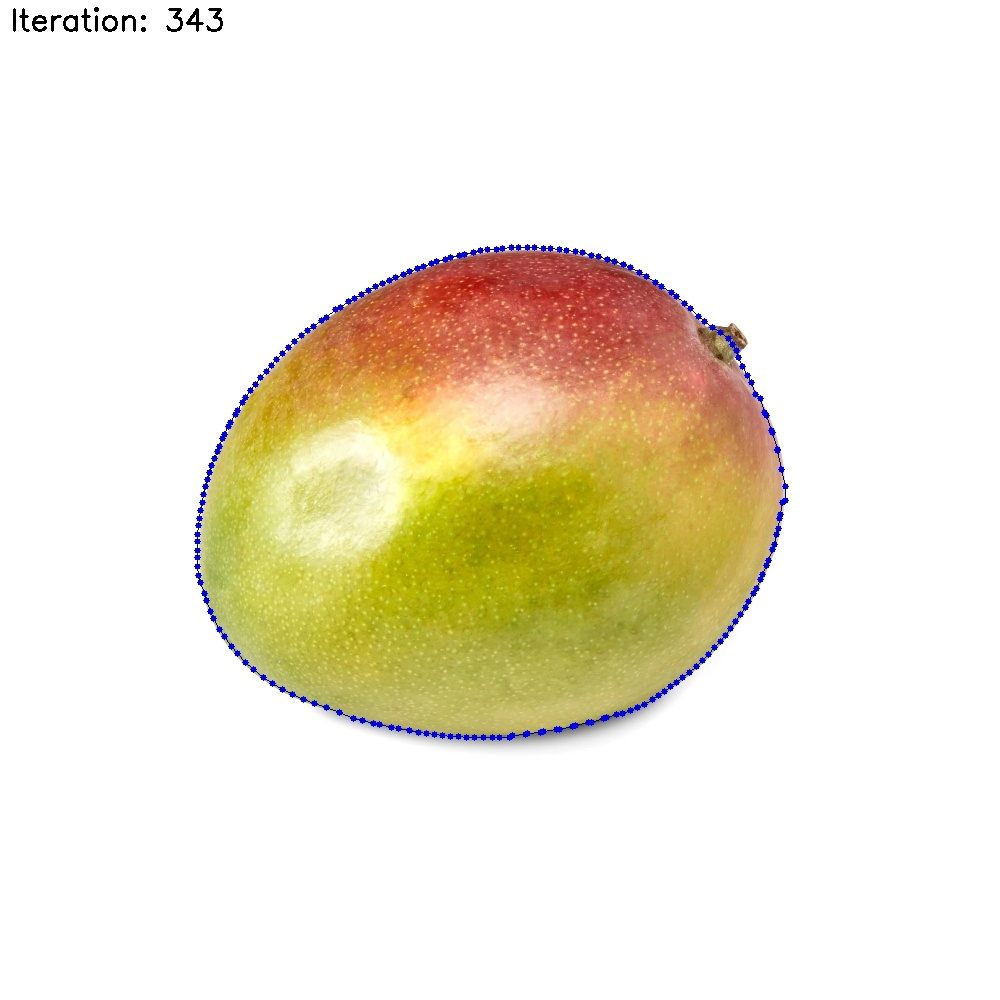
\includegraphics[height=0.3\paperheight]{result_img/result_img1.jpg}
    \caption{result images for img1.jpg}
\end{figure}
\begin{figure}[!htb]
    \centering
      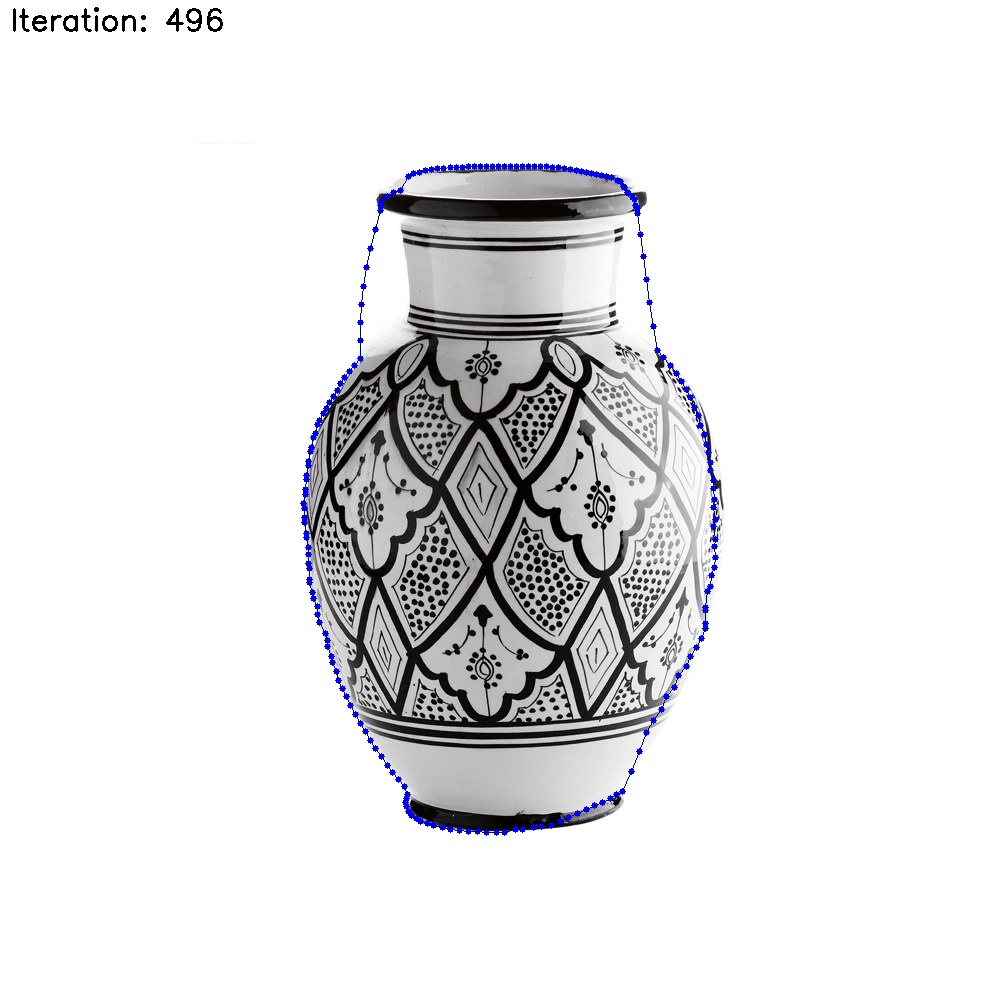
\includegraphics[height=0.3\paperheight]{result_img/result_img2.jpg}
    \caption{result images for img2.jpg}
\end{figure}
\begin{figure}[!htb]
    \centering
      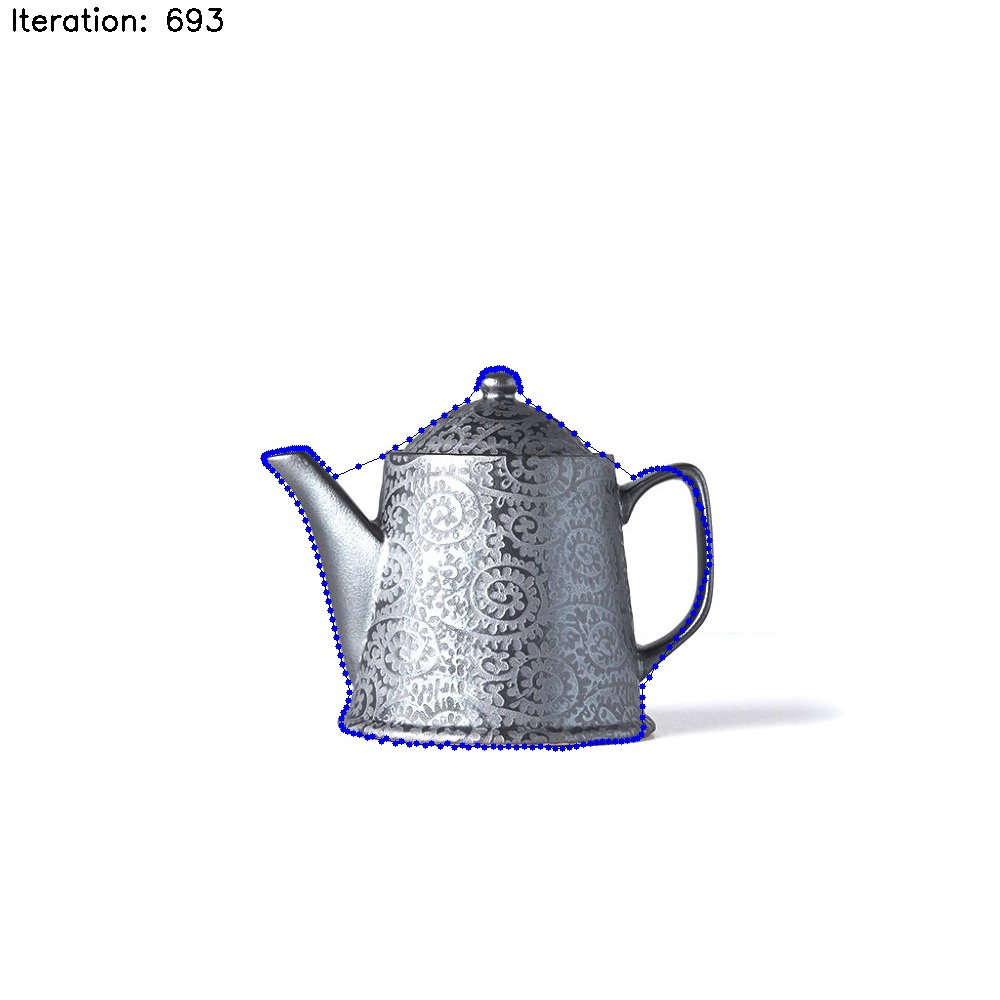
\includegraphics[height=0.3\paperheight]{result_img/result_img3.jpg}
    \caption{result images for img3.jpg}
\end{figure}


\clearpage
\section{Observations}
\subsection{Gaussian Filter}
\paragraph*{}
Gaussian blur is a method used in the active contour algorithm to smooth out images. It helps by reducing noise and removing rough edges and unnecessary details. This smoothing makes it easier for the algorithm to identify and track the outlines of objects in an image. However, it's important not to use too much Gaussian blur. If the image becomes overly blurred, the algorithm can become slower and lose important details. This loss of detail can make the algorithm less accurate in recognizing the shapes and features of the image. Therefore, it's crucial to use just the right amount of Gaussian blur to keep the algorithm working well.

\subsection{Image Preprocessing}
\paragraph*{}
Image preprocessing is a critical step in enhancing the overall performance of image analysis and processing tasks. In your specific example, the application of a lower threshold is used as a preprocessing technique. This approach plays a vital role in improving the accuracy and speed of the subsequent image processing tasks.
\paragraph*{}
By applying a lower threshold:
\begin{itemize}
    \item Unwanted low-intensity areas like shadows are filtered out, leading to a cleaner image.
    \item The resulting image has more pronounced features of interest.
\end{itemize}
\paragraph*{}
Benefits of lower thresholding in image preprocessing include:
\begin{itemize}
    \item \textbf{Increased Accuracy:} The removal of irrelevant data, like shadows, allows for more precise analysis of important image features.
    \item \textbf{Enhanced Speed:} Reducing the complexity and data points in the image decreases the computational load, allowing for faster processing in subsequent analysis stages.
\end{itemize}

\subsection{Initial Contour Setup}
\paragraph*{}
Initial contour point setup is crucial part. A well-thought-out setup can significantly enhance the efficiency of the algorithm. One effective approach is to use a circular initial contour. This method helps to mitigate the 'corner effect', where corners take longer time to converge, potentially slowing down the process. Alternatively, a rectangular initial contour can be used to ensure comprehensive coverage of the image area, especially in images where the target features are more aligned with rectangular shapes.

However, it's important to note that there is no one-size-fits-all solution for all problems. The effectiveness of the initial contour setup can be greatly improved by having prior knowledge about the target image, ideally supervised by a human. This allows for a more tailored approach, increasing the efficiency and accuracy of the image processing task.

In the context of this experiment, The circular model was chosen. The circle has a radius of 400 pixels, and its center coincides with the center of the image. This setup was chosen as it provides a balanced approach, offering good initial coverage and reducing the time to converge, especially in images where the target features are centrally located or distributed evenly across the image. This standardized approach simplifies the process and provides a consistent starting point for processing a variety of images

\subsection{Contour Point Searching Window Size}
\paragraph*{}
After conducting multiple experiments, it was determined that the optimal search window size is 25x25. In real-world applications, the choice of this parameter significantly depends on the gap between distinct features in an image and their intensity levels. The selection of an appropriate window size is critical for efficient processing. If the window size is too small, the algorithm might slow down or get stuck in local minima noise. This occurs because a smaller window may not capture enough context to make accurate decisions, leading to repeated recalculations or getting trapped in a suboptimal solution that appears best in a limited view but isn't globally optimal.\\
On the other hand, a window that's too large risks overlooking important features. Larger windows encompass more of the image, which can dilute the significance of smaller, yet critical features. This can cause the algorithm to miss subtle but essential details, as it focuses on broader trends over smaller, localized variations. In essence, the window size acts as a balancing factor. It must be large enough to capture sufficient context for accurate analysis but not so large that it overlooks finer details. Adjusting this parameter based on the feature gap and intensity ensures the algorithm remains sensitive to important details while maintaining processing efficiency.

\subsection{\(\alpha\), \(\beta\), and \(\gamma\) Selection}
\paragraph*{}
These parameters are crucial for balancing the internal and external forces acting on the contour and can significantly affect the behavior and effectiveness of the model.

\subsubsection*{Alpha (\(\alpha\)) - Continuity Term}
\paragraph*{Purpose:} 
This parameter controls the influence of the continuity energy term in the snake model. Continuity energy aims to maintain an even spacing between consecutive points on the contour, promoting a uniform distribution of points.
\paragraph*{Effect:}
A higher value of \(\alpha\) makes the contour act like a tightly stretched elastic band, resisting large differences in distance between adjacent points. This can prevent the contour from easily bending or adapting to complex shapes.
A lower value of \(\alpha\) allows more flexibility, enabling the contour to more easily conform to the object's shape but may lead to uneven point distribution or a less stable contour.

\subsubsection*{Beta (\(\beta\)) - Curvature Term:}
\paragraph*{Purpose:} 
Beta controls the curvature energy term, which penalizes sharp bends or curves in the contour. It encourages the contour to be smooth and less wavy.
\paragraph*{Effect:}
A high value of \(\beta\) results in a smoother contour, resisting sharp turns or bends. This can be helpful in ignoring small, irrelevant details or noise but may prevent the contour from accurately fitting into sharp corners or concave regions.
A low value of \(\beta\) allows the contour to have more bends and curves, which can be useful for outlining irregular or complex shapes, but it may also make the contour more susceptible to noise and small irrelevant details.

\subsubsection*{Gamma (\(\gamma\)) -  Proportion of Intensity (External) Energy:}
\paragraph*{Purpose:} 
Gamma controls the relative influence of the external energy term, which is often related to the image's intensity (such as edge information or other image features).
\paragraph*{Effect:}
A large \(\gamma\)  increases the influence of image-based features (like edges) on the movement of the contour. This can help the contour to better adhere to prominent image features.
A smaller \(\gamma\) reduces the impact of image intensity on the contour, making internal forces (like continuity and curvature) more dominant. This might be useful in situations where the internal structure of the contour is more important than the exact image features.
\paragraph*{}
Balancing these parameters is key to achieving good performance with active contours. The optimal values often depend on the specific characteristics of the image and the object being segmented. For instance, images with well-defined edges might require different parameter settings than those with more subtle or textured boundaries. Experimentation and tuning are usually necessary to find the most effective combination of \(\alpha\), \(\beta\), and \(\gamma\) for a given application.
\begin{figure}[!]
    \begin{minipage}{\linewidth}
        \centering
        \begin{subfigure}{0.49\textwidth}
              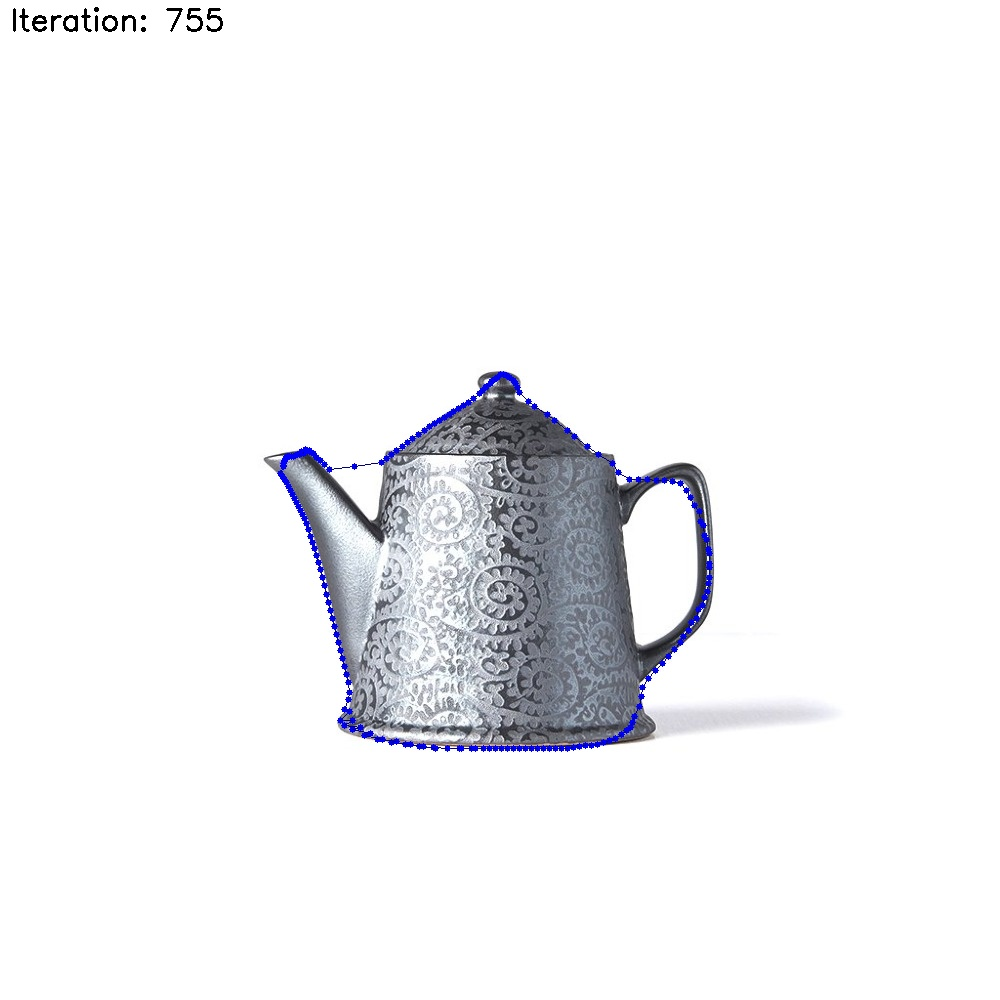
\includegraphics[width=\linewidth]{result_img/beta_0_01.jpg}
            \subcaption{\(\beta\)=0.01}
        \end{subfigure}
        \begin{subfigure}{0.49\textwidth}
              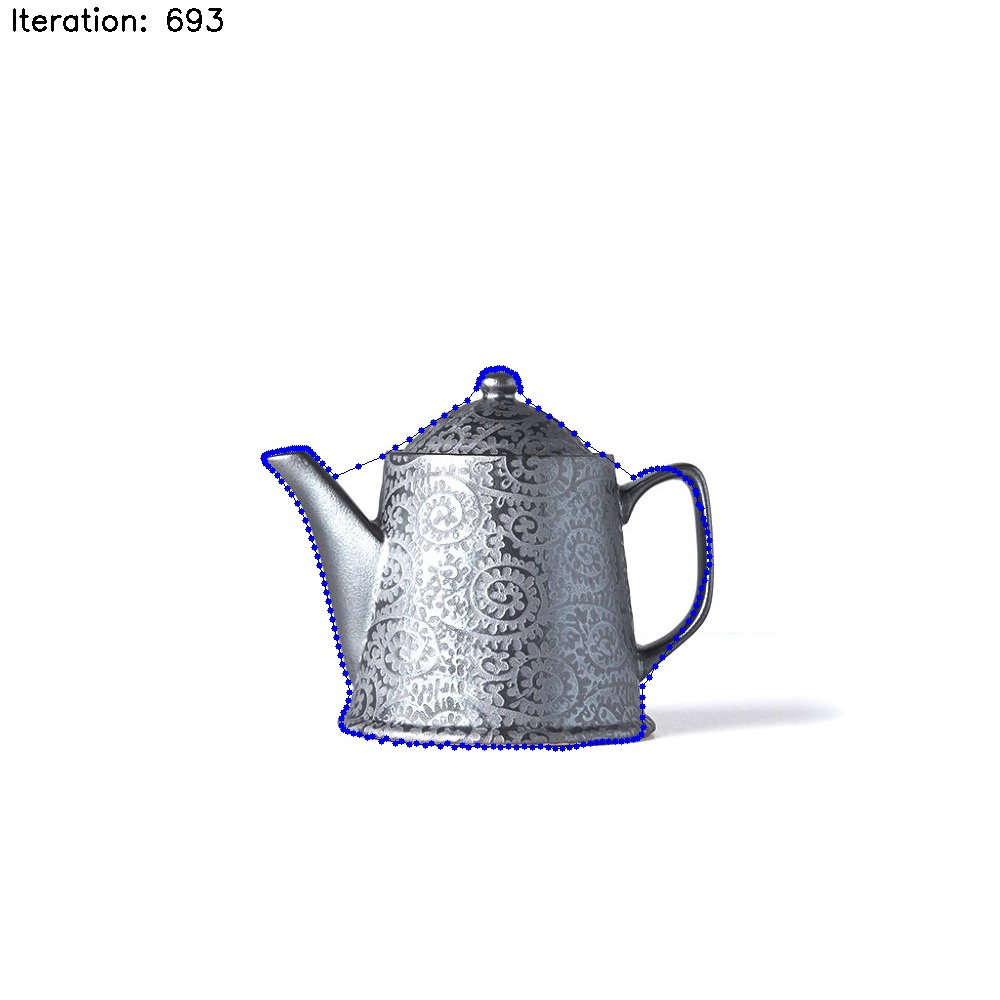
\includegraphics[width=\linewidth]{result_img/beta_0_00001.jpg}
            \subcaption{\(\beta\)=0.00001}
        \end{subfigure}

        \caption{Curvature Term \(\beta\) affects the result}
    \end{minipage}

\end{figure}


\subsection{Convergence Detection, Oscillating State, and Terminal Condition}
\paragraph*{}
For this experiment, we have chosen to use 'convergence' or 'oscillation' as the terminal criteria. Convergence is defined as the point where the movement of the contour points becomes negligible, indicating that the algorithm has successfully detected the target features and there is no further significant change in the contour's position. This is a common criterion in image processing, as it signifies that the algorithm has stabilized and the desired outcome has been achieved.
\paragraph*{}
On the other hand, 'oscillation' is used as a criterion to prevent excessive computation and to handle cases where the contour cannot settle on a stable configuration. Oscillation occurs when the contour points repeatedly move back and forth over a small area without reaching a state of convergence. When such a pattern is detected, the process is terminated to avoid unnecessary calculations and potential infinite loops.
\paragraph*{}
By employing these two criteria, we ensure that the experiment is efficient and effective. The use of convergence as a terminal point guarantees accuracy in stable scenarios, while the incorporation of oscillation as a criterion safeguards against computational inefficiency in more complex or problematic cases.

\subsection{Gradient Vector Field}
\paragraph*{}
The use of a gradient vector field in image processing is an effective approach, especially in tasks like contour detection. However, relying solely on first-order derivatives (the rate of change of intensity) presents certain limitations. In the first-order gradient, the direction of the gradient vectors points outward from the edges in the image, indicating the direction in which intensity increases. When these gradients are used to move contour points, they provide a force that attracts these points towards areas of higher intensity. This works well up to the edge of an object, but the issue arises once the contour point crosses the edge.
\paragraph*{}
The primary problem with first-order gradients is their lack of an attracting force back towards the edge once a contour point has passed it. This means if a point overshoots the edge, the first-order gradient doesn't provide the necessary information to guide it back, resulting in incorrect positioning of the contour. This behavior leads to inaccuracies in accurately tracing the object's boundaries.
\paragraph*{}
Switching to second-order derivatives can address this issue effectively. The second-order gradient doesn't just indicate the rate of change of intensity but also the rate at which this rate of change is itself changing. This additional information is crucial as it can indicate where the intensity changes are beginning to decrease, essentially highlighting the edges more effectively. When a contour point crosses an edge, the second-order gradient provides a signal that the point is moving away from a region of rapid intensity change, thus encouraging a return to the edge. This mechanism ensures a more accurate and reliable contour detection, as the points are better guided to conform to the actual edges of objects in the image. The effectiveness of second-order gradients over first-order ones in this context is often illustrated in comparative images, showing how they better capture the true edges and contours in various scenarios.

\begin{figure}[!]
    \begin{minipage}{\linewidth}
        \centering
        \begin{subfigure}{0.49\textwidth}
              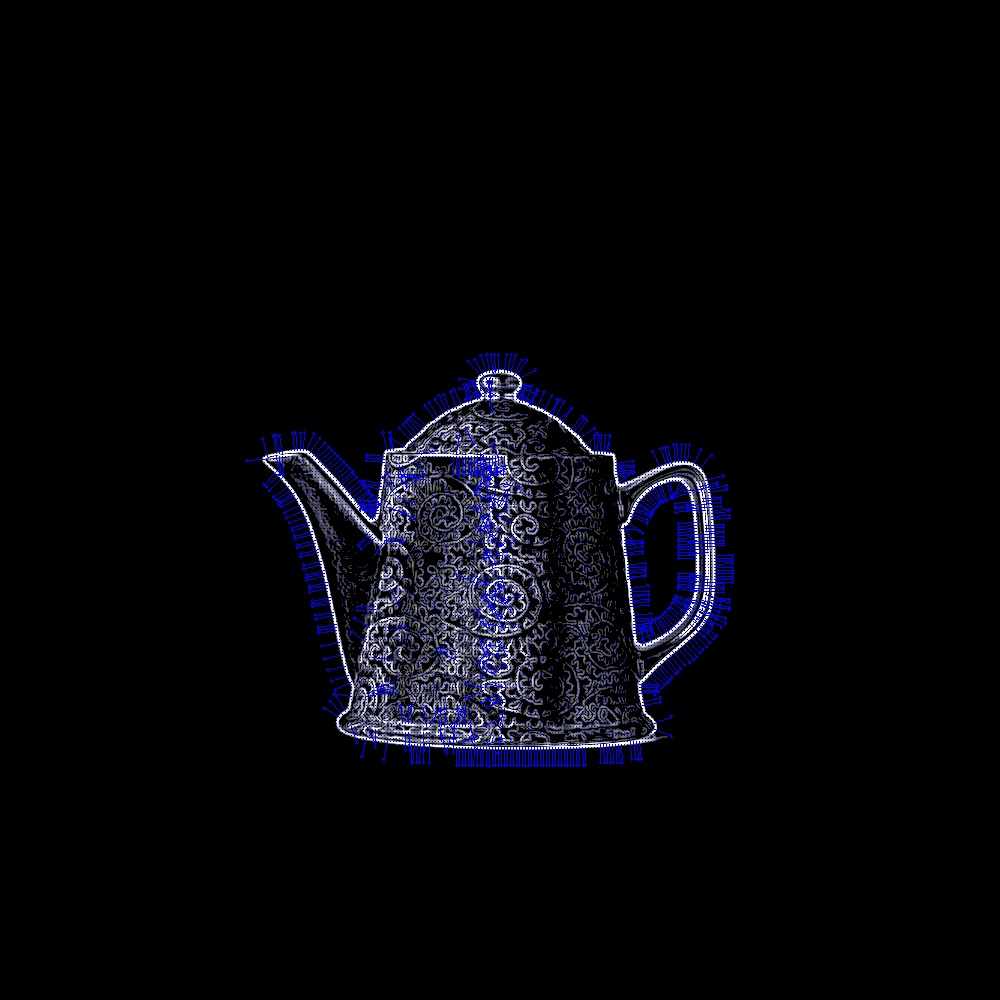
\includegraphics[width=\linewidth]{output/first_order_gvf.jpg}
            \subcaption{First Order}
        \end{subfigure}
        \begin{subfigure}{0.49\textwidth}
              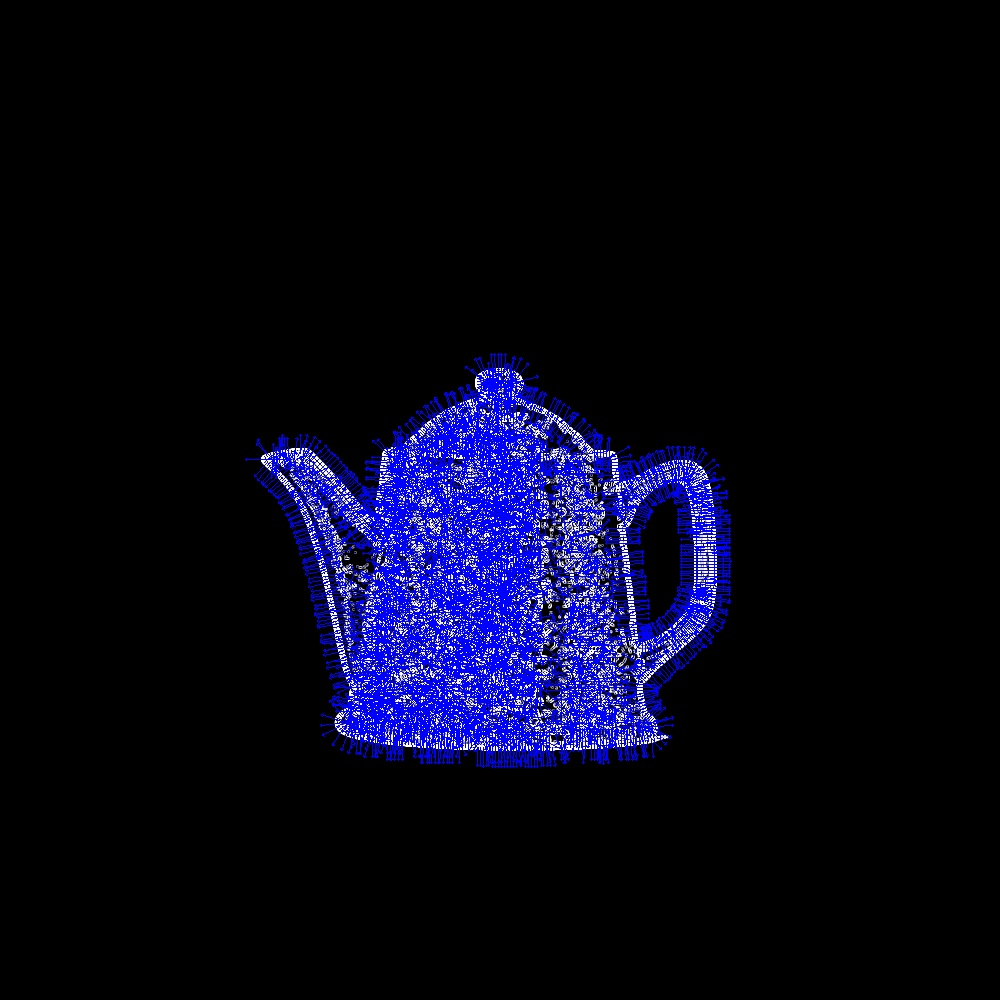
\includegraphics[width=\linewidth]{output/second_order_gvf.jpg}
            \subcaption{Second Order}
        \end{subfigure}

        \caption{Comparison between first order and second order GVF}
    \end{minipage}

\end{figure}

\clearpage

\subsection{Force Model}
\paragraph*{}
There is an alternative approach for moving contour points: the force model. While the energy model is more traditional, using a force model can offer distinct advantages, particularly in terms of convergence speed and computational efficiency.
\paragraph*{}
The force model, unlike the energy model, does not rely on the size of a search window. This independence from window size is a significant advantage because it eliminates the need to optimize this parameter, which can be both time-consuming and computationally expensive. By not being tied to a search window, the force model can converge more rapidly to the desired solution, as it is less constrained and can react more directly to the image data.
\paragraph*{}
Another benefit of the force model is its reduced computational load. Since it doesn't depend on iteratively scanning through various window sizes, the number of calculations required is substantially lower. This makes the process faster and more efficient, particularly for larger images or more complex contours.
\paragraph*{}
The force model operates through vector addition. In this approach, forces are calculated at each contour point, and these forces are then summed up (or integrated) to determine the direction and magnitude of movement for each point. This method is more dynamic and can adapt quickly to changes in the image data.
\paragraph*{}
Gradient Vector Flow (GVF) plays a crucial role in this force model, both in its first-order and second-order forms. First-order GVF provides information about the direction of the most significant intensity change, guiding the contour points towards areas of high gradient. Second-order GVF, on the other hand, adds context about the curvature of the intensity landscape, helping to more accurately target the edges of objects.
\paragraph*{}
While in this homework, the code for this approach is not provided since it is still not provide a good result and I decided to remove it, the experiments was conducted, and the potential of this method is clear. Its faster convergence and reduced computational.

\begin{figure}[!htb]
    \begin{minipage}{\linewidth}
        \centering
        \begin{subfigure}{0.49\textwidth}
            %   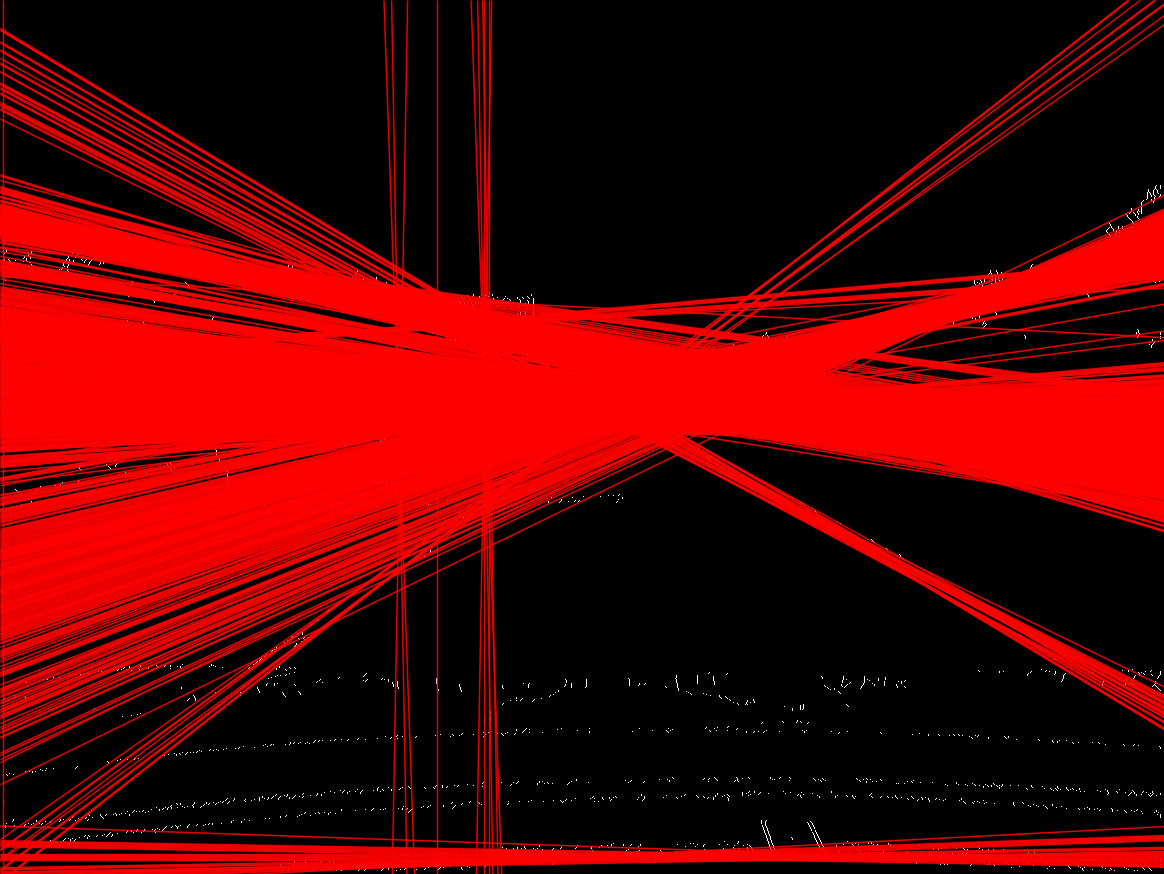
\includegraphics[width=\linewidth]{output/img2_q3_HOUGH_THETA_1_THRES_50.png}
            \subcaption{Theta = 1 deg}
        \end{subfigure}
        \begin{subfigure}{0.49\textwidth}
            %   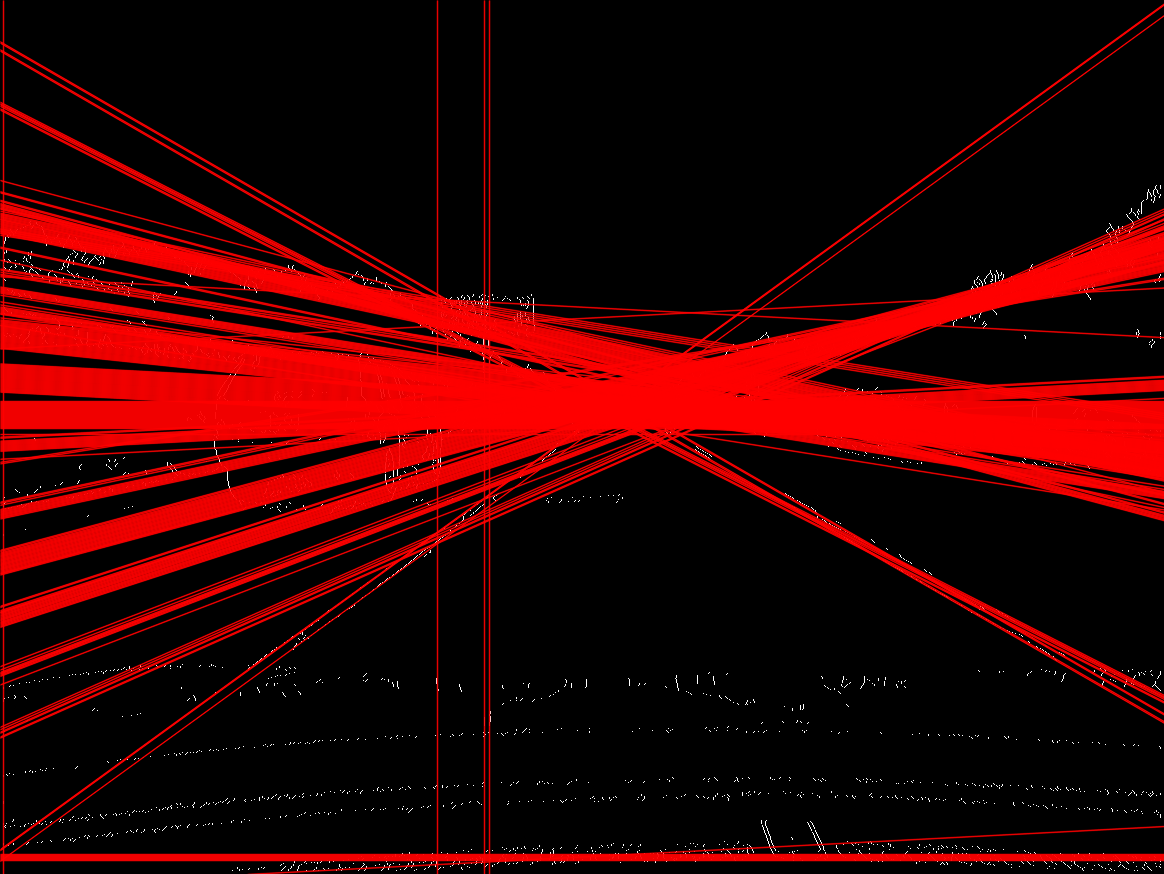
\includegraphics[width=\linewidth]{output/img2_q3_HOUGH_THETA_3_THRES_50.png}
            \subcaption{Theta = 3 deg}
        \end{subfigure}

        \begin{subfigure}{0.49\textwidth}
            %   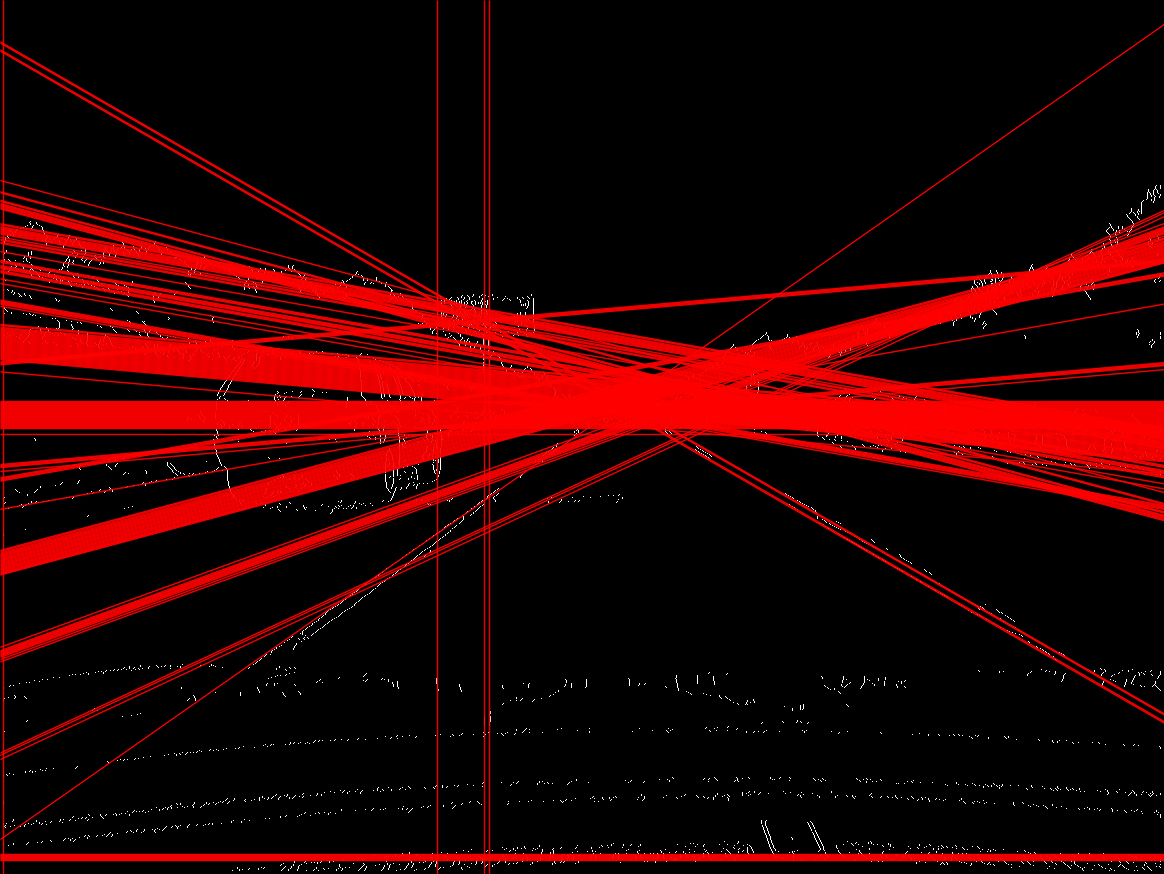
\includegraphics[width=\linewidth]{output/img2_q3_HOUGH_THETA_5_THRES_50.png}
            \subcaption{Theta = 5 deg}
        \end{subfigure}
        \begin{subfigure}{0.49\textwidth}
            %   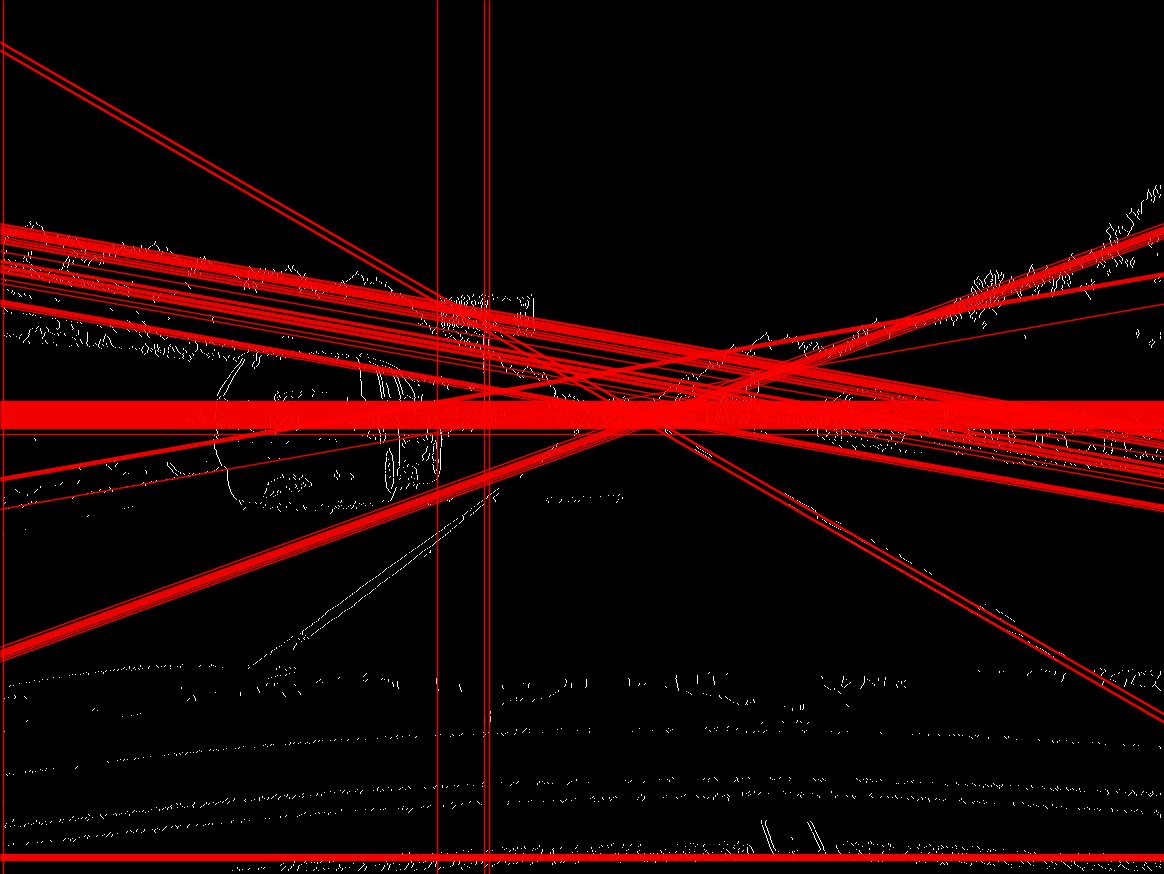
\includegraphics[width=\linewidth]{output/img2_q3_HOUGH_THETA_10_THRES_50.png}
            \subcaption{Theta = 10 deg}
        \end{subfigure}

        \caption{Comparison of Angle step affect line detection}
    \end{minipage}

\end{figure}

\clearpage

\subsection{Summary}
\paragraph*{}Please be reminded that there is no single, complete formula that yields the best
result. For this case, prior knowledge about the line direction helps increase accuracy and reduce calculation complexity

\appendix
\chapter{Git Repository}

\verb|Git Repository: chinatip-l/computer-vision-lab-fall-2023| \\
URL: \url{https://github.com/chinatip-l/computer-vision-lab-fall-2023}

\chapter{Source Code: main.cpp}
\begin{lstlisting}
#include <stdio.h>
#include <opencv2/opencv.hpp>
#include <unistd.h>
#include <string.h>
#include "include/func.hpp"
#include <opencv2/videoio/videoio_c.h>

#define MAX_LEN 250

// path for lab
#define BASE_PATH "/home/chinatip/computer-vision-lab-fall-2023/homework4"
#define SRC_PATH "test_img"
#define OUT_PATH "output"

// define file name, can uncomment to select the input
#define FILENAME "img1"
// #define FILENAME "img2"
// #define FILENAME "img3"

#define EXT "jpg"

Mat canvas;

void appendImgToCanvas(Mat);

int main(int argc, char **argv)
{

    Mat og_img;
    char og_file[MAX_LEN] = "", out_file[MAX_LEN] = "";
    snprintf(og_file, MAX_LEN, "%s/%s/%s.%s", BASE_PATH, SRC_PATH, FILENAME, EXT);

    og_img = imread(og_file);

    if (!og_img.data)
    {
        printf("No image data \n");
        return -1;
    }
    else
    {
        printf("Original Img Size: w x h %d x %d\n", og_img.cols, og_img.rows);
    }

    appendImgToCanvas(og_img);
    Mat bw_img;
    bw_img = applyGreyscaleFilter(og_img);

    Mat res_img, selected_img;

    Mat gaussian_filter = createGaussianFilter(3, 1);
    res_img = applyFilter(bw_img, gaussian_filter, 1, false);
    printf("Gaussian Filter Img Size: w x h %d x %d\n", res_img.cols, res_img.rows);

    appendImgToCanvas(res_img);

    Mat sobelx;
    sobelx = applySobelX(res_img);
    appendImgToCanvas(sobelx);

    Mat sobely;
    sobely = applySobelY(res_img);
    appendImgToCanvas(sobely);

    Mat magnitude;
    magnitude = calculateEdgeStrength(sobelx, sobely);

    Mat direction;
    direction = calculateEdgeDirection(sobelx, sobely);

    Mat output;
    magnitude.copyTo(output);
    showGradient(output, magnitude, direction, 3);
    snprintf(out_file, MAX_LEN, "%s/%s/first_order_gvf.jpg", BASE_PATH, OUT_PATH);
    imwrite(out_file, output);

    Mat mag2, dir2, dx, dy, res;
    dx = applySobelX(magnitude);
    dy = applySobelY(magnitude);
    mag2 = calculateEdgeStrength(dx, dy);
    dir2 = calculateEdgeDirection(dx, dy);

    mag2.copyTo(output);
    showGradient(output, mag2, dir2, 3);
    snprintf(out_file, MAX_LEN, "%s/%s/second_order_gvf.jpg", BASE_PATH, OUT_PATH);
    imwrite(out_file, output);

    vector<ContourPoint> contour;

    VideoWriter video;
    char video_name[100] = "\0";
    snprintf(video_name, 99, "%s/%s/vid_%s.mp4", BASE_PATH, OUT_PATH, FILENAME);
    video.open(video_name, CV_FOURCC('m', 'p', '4', 'v'), 10, og_img.size(), true);

    // We apply termination logic outside the active contour function
    // it is done by calculate energy over 4 last epochs
    // if it oscillates or stable, we increase count by 1
    // The threshold of count is 20 to help avoid local minima

    contour = initContourPointCircle(magnitude.cols / 2, magnitude.rows / 2, 400, 200);
    float alpha = 0.05, beta = 0.00001, gamma = 0.5;
    float min_e = numeric_limits<float>::max(), current_e, e_1 = 0, e_2 = 0, e_3 = 0, e_4 = 0, diff1, diff2, diff3;
    bool isOscillating = false, isConverging = false;
    int osc_cnt = 0;
    vector<Mat> buf;
    char iter_text[25] = "\0";
    for (int k = 0; k < 10000; k++)
    {
        Mat i;
        activeContour(mag2, dir2, contour, alpha, beta, gamma);
        current_e = contourEnergy(contour);

        Mat mag_with_field;
        og_img.copyTo(mag_with_field);
        i = showSnake(mag_with_field, contour);

        // calculate energy over 4 latest energy to check
        // if converge or oscillate
        e_4 = e_3;
        e_3 = e_2;
        e_2 = e_1;
        e_1 = current_e;
        diff1 = e_2 - e_1;
        diff2 = e_3 - e_2;
        diff3 = e_4 - e_3;
        isOscillating = (diff1 * diff2 < 0) && (diff2 * diff3 < 0);
        isConverging = std::abs(diff1) == std::abs(diff2) && std::abs(diff2) == std::abs(diff3);

        if (!(isOscillating && isConverging))
        {
            min_e = current_e;
            osc_cnt = 0;
        }
        else
        {
            osc_cnt += 1;
            // termination condition
            if (osc_cnt == 20)
            {

                snprintf(iter_text, 24, "Iteration: %d", k);
                putText(i, iter_text, Point2i(10, 30), FONT_HERSHEY_SIMPLEX, 1, (0, 0, 0), 2);
                printf("Frame %d %f\n", k, min_e);
                snprintf(out_file, MAX_LEN, "%s/%s/result_%s.%s", BASE_PATH, OUT_PATH, FILENAME, EXT);
                imwrite(out_file, i);
                imshow("Original", i);
                video.write(i);
                video.release();
                waitKey(10);
                break;
            }
        }

        if (k % 10 == 0)
        {
            snprintf(iter_text, 24, "Iteration: %d", k);
            putText(i, iter_text, Point2i(10, 30), FONT_HERSHEY_SIMPLEX, 1, (0, 0, 0), 2);
            imshow("Original", i);
            video.write(i);
            waitKey(10);
        }
    }
    printf("Finish\n");
    waitKey(0);
    return 0;
}

void appendImgToCanvas(Mat img)
{
    if (canvas.empty())
    {
        canvas = img;
    }
    else
    {
        Size s(canvas.cols + img.cols + 5, canvas.rows > img.rows ? canvas.rows : img.rows);
        size_t old_w = canvas.cols;
        copyMakeBorder(canvas, canvas, 0, 0, 0, img.cols + 5, BORDER_CONSTANT, Scalar(0, 0, 0, 0));
        img.copyTo(canvas(Rect(old_w + 5, 0, img.cols, img.rows)));
    }
}

\end{lstlisting}

\chapter{Source Code: func.hpp}
\begin{lstlisting}
#ifndef _FUNC_H_
#define _FUNC_H_

#include <opencv2/opencv.hpp>
#include <vector>

using namespace cv;
using namespace std;

/**
* @brief Class representing a point with additional energy attribute.
*
* Inherits from OpenCV's Point2f class and adds an energy attribute.
* This can be used to represent points in an image with an associated energy value.
*/
class ContourPoint : public Point2f
{
public:
float energy; ///< Energy value of the contour point.
};

/**
* @brief Applies a greyscale filter to an image.
*
* @param image The source image to be converted.
* @return Grayscale version of the input image.
*/
Mat applyGreyscaleFilter(Mat image);

/**
* @brief Calculates Gaussian value for given coordinates and sigma.
*
* @param x X-coordinate.
* @param y Y-coordinate.
* @param sigma Standard deviation of the Gaussian function.
* @return Gaussian value for the specified coordinates and sigma.
*/
float calculateGaussian(int x, int y, float sigma);

/**
* @brief Creates a Gaussian filter kernel of a specified size and sigma.
*
* @param size Size of the Gaussian filter (typically odd number).
* @param sigma Standard deviation of the Gaussian.
* @return Gaussian filter as a Mat object.
*/
Mat createGaussianFilter(int size, float sigma);

/**
* @brief Applies a filter to an image with optional border suppression.
*
* @param image The source image.
* @param kernel The filter kernel.
* @param stride Stride for the convolution.
* @param suppress_border If true, suppresses the border effects.
* @return The filtered image.
*/
Mat applyFilter(Mat image, Mat kernel, int stride, bool suppress_border);

/**
* @brief Applies the Sobel operator in the X direction.
*
* @param image The source image.
* @return Image after applying the Sobel X operator.
*/
Mat applySobelX(Mat image);

/**
* @brief Applies the Sobel operator in the Y direction.
*
* @param image The source image.
* @return Image after applying the Sobel Y operator.
*/
Mat applySobelY(Mat image);

/**
* @brief Calculates the edge strength from gradient images.
*
* @param grad_x Gradient image in the X direction.
* @param grad_y Gradient image in the Y direction.
* @return Edge strength image.
*/
Mat calculateEdgeStrength(Mat grad_x, Mat grad_y);

/**
* @brief Calculates the edge direction from gradient images.
*
* @param grad_x Gradient image in the X direction.
* @param grad_y Gradient image in the Y direction.
* @return Edge direction image.
*/
Mat calculateEdgeDirection(Mat grad_x, Mat grad_y);

/**
* @brief Initialises contour points in a circular pattern.
*
* @param cx X-coordinate of the circle center.
* @param cy Y-coordinate of the circle center.
* @param r Radius of the circle.
* @param quantity Number of contour points to generate.
* @return Vector of initialised contour points.
*/
vector<ContourPoint> initContourPointCircle(int cx, int cy, int r, int quantity);

/**
* @brief Implements the active contour model (snake) algorithm.
*
* @param magnitude Magnitude of the gradient.
* @param direction Direction of the gradient.
* @param contour Reference to a vector of ContourPoints representing the snake.
* @param alpha Weight for continuity energy.
* @param beta Weight for curvature energy.
* @param gamma Weight for image energy.
*/
void activeContour(Mat magnitude, Mat direction, vector<ContourPoint> &contour, float alpha, float beta, float gamma);

/**
* @brief Calculates the total energy of a contour.
*
* @param contour Vector of ContourPoints.
* @return Total energy of the contour.
*/
float contourEnergy(vector<ContourPoint> &contour);

/**
* @brief Visualises the snake on an image.
*
* @param image The source image.
* @param contour Vector of ContourPoints representing the snake.
* @return Image with the snake visualised.
*/
Mat showSnake(Mat image, vector<ContourPoint> contour);

/**
* @brief Displays gradient information on an image.
*
* @param image Reference to the source image.
* @param magnitude Gradient magnitude.
* @param direction Gradient direction.
* @param stride Stride for visualization.
*/
void showGradient(Mat &image, Mat magnitude, Mat direction, int stride);

#endif // _FUNC_H_

\end{lstlisting}

\chapter{Source Code: func.cpp}
\begin{lstlisting}
#include "include/func.hpp"
#include <vector>
#include <cmath>
#include <limits>

const double K_E = std::exp(1.0);

Mat applyGreyscaleFilter(Mat img)
{
    // Create New Image as Output Image
    Mat bw_img(img.size(), img.type());
    for (int j = 0; j < img.rows; j++)
    {
        for (int i = 0; i < img.cols; i++)
        {
            // Get the pixel value from the original image
            Vec3b brg_px = img.at<Vec3b>(j, i);

            // Normal average function ie. sum(xn)/n ;
            int b = (brg_px[0] + brg_px[1] + brg_px[2]) / 3;

            // Write back to every channel
            brg_px[0] = b;
            brg_px[1] = b;
            brg_px[2] = b;

            // Write to new image buffer
            bw_img.at<Vec3b>(j, i) = brg_px;
        }
    }
    // return the output image
    return bw_img;
}

float calculateGaussian(int x, int y, float sigma)
{
    return (1 / (CV_2PI * sigma * sigma)) * (powf32(K_E, -1 * ((x * x) + (y * y)) / (2 * sigma * sigma)));
}

Mat createGaussianFilter(int size, float sigma)
{
    int center = size / 2;
    Mat kernel = Mat::zeros(size, size, CV_32F);
    for (int j = 0; j < kernel.rows; j++)
    {
        for (int i = 0; i < kernel.cols; i++)
        {
            kernel.at<float>(j, i) = calculateGaussian(i - center, j - center, sigma);
        }
    }
    return kernel;
}

Mat applyFilter(Mat img, Mat kernel, int stride, bool suppress_border)
{

    // calculate kernel offset ie. number of pixel before and
    // after since the target pixel will be the center of
    // matrix,
    // in order to get the neighbour pixel with size of kernel
    // size, offset will be applied for both before, and after
    // the target pixel
    // example
    // width = 5 => offset = (int)5/2 = 2;
    // px   ... k   n-offset    ... n   ... n+offset    k
    int ker_x_offset = kernel.cols / 2;
    int ker_y_offset = kernel.rows / 2;

    int padding = ker_x_offset;

    // get kernel size
    int ker_w = kernel.cols;
    int ker_h = kernel.rows;

    // calculate output image size
    int out_w = ((img.cols + (2 * padding) - kernel.cols) / stride) + 1;
    int out_h = ((img.rows + (2 * padding) - kernel.rows) / stride) + 1;

    // create intermediate buffer and add padding, size is
    // w+(2*padding),h+(2*padding) then copy the content
    // of image to the buffer
    Mat padded;
    padded = Mat::zeros(img.rows + (2 * padding), img.cols + (2 * padding), CV_32SC3);
    int dtype = img.type();

    // here, we convert data type while copy to make it compatible
    // for higher precision computation
    // check if input is uint8 or int 32
    // if uint8 then we will channel-wise copy to padded buffer
    // due to different data alignment
    // if int38 then we will pixel-wise copy to padded buffer
    switch (dtype)
    {
    case CV_32SC3:
        for (int j = 0; j < img.rows; j++)
        {
            for (int i = 0; i < img.cols; i++)
            {
                padded.at<Vec3i>(j + padding, i + padding) = img.at<Vec3i>(j, i);
            }
        }
        break;
    case CV_8UC3:
        for (int j = 0; j < img.rows; j++)
        {
            for (int i = 0; i < img.cols; i++)
            {
                for (int k = 0; k < 3; k++)
                {
                    padded.at<Vec3i>(j + padding, i + padding)[k] = img.at<Vec3b>(j, i)[k];
                }
            }
        }
        break;
    default:
        break;
    }

    // create output buffer with calculated output size
    // data type need to be vector of signed int 32 bit
    // in case negative data is possible, this can help
    // preserve information through the convolution process
    // and rasterise to 8 bit at the last step
    Mat img_res = Mat::zeros(out_h, out_w, CV_32SC3);

    Vec3i res(0, 0, 0);

    // iterate over the size of input image
    for (int img_j = 0; img_j < img.rows; img_j += stride)
    {
        for (int img_i = 0; img_i < img.cols; img_i += stride)
        {
            // check if it is a border and suppress border
            // if selected
            if (img_i < ker_w || img_j < ker_h || img_i > img.cols - ker_h - 1 || img_j > img.rows - ker_h - 1)
            {
                if (suppress_border)
                {
                    res = Vec3i(0, 0, 0);
                    img_res.at<Vec3i>((img_j) / stride, (img_i) / stride) = res;
                    continue;
                }
            }

            // get windowed matrix from the padded buffer with
            // the size of kernel size, and target pixel is in
            // the center of windowed matrix
            Mat windowed = padded(Rect(img_i, img_j, ker_w, ker_h));
            res = Vec3i(0, 0, 0);
            float tmp = 0;
            float tmp1 = 0;
            float tmp2 = 0;
            float tmp3 = 0;

            // item-wise multiply windowed matrix with kernel
            // matrix and summarise
            for (int ker_j = 0; ker_j < kernel.rows; ker_j++)
            {
                for (int ker_i = 0; ker_i < kernel.cols; ker_i++)
                {
                    Vec3b t = windowed.at<Vec3i>(ker_j, ker_i);
                    float k = kernel.at<float>(ker_j, ker_i);
                    tmp += (t[0] * k);
                    tmp1 += (t[0] * k);
                    tmp2 += (t[1] * k);
                    tmp3 += (t[2] * k);
                }
            }
            res[0] = tmp1;
            res[1] = tmp2;
            res[2] = tmp3;

            // write to output buffer
            img_res.at<Vec3i>((img_j) / stride, (img_i) / stride) = res;
        }
    }
    // return the output image
    return img_res;
}

Mat applySobelX(Mat img_in)
{
    float c_sobelX[] = {-1, 0, 1,
                        -2, 0, 2,
                        -1, 0, 1};
    Mat sobelX(3, 3, CV_32F, c_sobelX);
    Mat result = applyFilter(img_in, sobelX, 1, true);
    return result;
}

Mat applySobelY(Mat img_in)
{
    float c_sobelY[] = {-1, -2, -1,
                        0, 0, 0,
                        1, 2, 1};
    Mat sobelY(3, 3, CV_32F, c_sobelY);
    Mat result = applyFilter(img_in, sobelY, 1, true);
    return result;
}

Mat calculateEdgeStrength(Mat grad_x, Mat grad_y)
{
    Mat strength = Mat::zeros(grad_x.rows, grad_x.cols, CV_8UC3);
    float tmp = 0;
    for (int j = 0; j < strength.rows; j += 1)
    {
        for (int i = 0; i < strength.cols; i += 1)
        {
            for (int k = 0; k < 3; k++)
            {
                // Strength of pixel is calculated by
                // sqrt(gx^2 + gy^2)
                tmp = (grad_x.at<Vec3i>(j, i)[k] * grad_x.at<Vec3i>(j, i)[k]) + (grad_y.at<Vec3i>(j, i)[k] * grad_y.at<Vec3i>(j, i)[k]);
                tmp = round(sqrtf32(tmp));

                // add clipping criteria in case of over 255
                // and lower bound for suppressing soft area
                if (tmp > 255)
                {
                    tmp = 255;
                }
                if (tmp < 50)
                {
                    tmp = 0;
                }
                strength.at<Vec3b>(j, i)[k] = (int)tmp;
            }
        }
    }

    return strength;
}

Mat calculateEdgeDirection(Mat grad_x, Mat grad_y)
{
    Mat direction = Mat::zeros(grad_x.rows, grad_x.cols, CV_32FC3);
    for (int j = 0; j < direction.rows; j += 1)
    {
        for (int i = 0; i < direction.cols; i += 1)
        {
            for (int k = 0; k < 3; k++)
            {
                // direction of pixel is calculated by
                // atan(y/x)
                direction.at<Vec3f>(j, i)[k] = atan2f32(grad_y.at<Vec3i>(j, i)[k], grad_x.at<Vec3i>(j, i)[k]);
            }
        }
    }
    return direction;
}

/**
    * @brief Initialise contour points in a circular pattern.
    *
    * This function creates a set of contour points arranged in the shape of a circle.
    * It is useful for initializing contour-based algorithms, especially for circular objects.
    *
    * @param cx The x-coordinate of the circle's center.
    * @param cy The y-coordinate of the circle's center.
    * @param r The radius of the circle.
    * @param quantity The number of contour points to generate.
    * @return vector<ContourPoint> A vector of contour points arranged in a circular pattern.
    */
vector<ContourPoint> initContourPointCircle(int cx, int cy, int r, int quantity)
{
    vector<ContourPoint> tmp;
    float theta = 0, d_theta = (2 * CV_PI) / quantity;

    for (int i = 0; i < quantity; i++)
    {
        float x, y;
        // Calculate the x and y coordinates using polar to
        // Cartesian conversion
        x = (r * cosf32(theta)) + cx;
        y = (r * sinf32(theta)) + cy;

        // Create a ContourPoint and set its properties
        ContourPoint p;
        p.x = x;
        p.y = y;

        // Since we try to minimise the energy, we initialise
        // the energy to the maximum float value
        p.energy = numeric_limits<float>::max();

        // Add the ContourPoint to the vector
        tmp.push_back(p);
        theta += d_theta;
    }

    // Return the vector of contour points
    return tmp;
}

/**
    * @brief Perform the active contour (snake) algorithm on an image.
    *
    * This function iteratively adjusts the positions of contour points to align with image features
    * like edges, based on an energy minimization process. The energy terms include continuity,
    * curvature, and image forces.
    *
    * @param magnitude The magnitude of the gradient of the image.
    * @param direction The direction of the gradient of the image.
    * @param contour A reference to a vector of ContourPoint representing the initial contour.
    * @param alpha The weight for the continuity energy term.
    * @param beta The weight for the curvature energy term.
    * @param gamma The weight for the image energy term.
    */
void activeContour(Mat magnitude, Mat direction, vector<ContourPoint> &contour, float alpha, float beta, float gamma)
{
    int p_cnt = contour.size();
    vector<ContourPoint> prev_contour(contour);

    for (int i = 0; i < p_cnt; i++)
    {
        // Retrieve previous, current, and next points in the contour
        ContourPoint pp, p, pn;
        pp = prev_contour[(i - 1 + p_cnt) % p_cnt];
        p = prev_contour[i % p_cnt];
        pn = prev_contour[(i + 1) % p_cnt];

        // Energy terms
        float e_cont, e_curve, e_image, e_point;

        // Search window settings
        int s_size = 25, s_offset = s_size / 2;
        int min_i = 0, min_j = 0;
        float min_e_point = numeric_limits<float>::max();

        // Search within the window to minimise energy
        for (int wj = 0; wj < s_size; wj++)
        {
            for (int wi = 0; wi < s_size; wi++)
            {
                ContourPoint tmp;

                // Candidate point within the window
                tmp.x = p.x - s_offset + wi;
                tmp.y = p.y - s_offset + wj;
                int tmp_mag = magnitude.at<Vec3b>((int)tmp.y, (int)tmp.x)[0];

                // Calculate energy terms
                e_cont = powf32((pn + pp - 2 * tmp).x, 2) + powf32((pn + pp - 2 * tmp).y, 2);
                e_curve = powf32((tmp - pp).x, 2) + powf32((tmp - pp).y, 2);
                e_image = -tmp_mag * tmp_mag;
                e_point = (alpha * e_cont) + (beta * e_curve) + (gamma * e_image);

                // Update if a lower energy point is found
                if (e_point < min_e_point)
                {
                    min_e_point = e_point;
                    min_i = tmp.x;
                    min_j = tmp.y;
                }
            }
        }

        // Update the contour point with the minimum energy point found
        contour[i].x = min_i;
        contour[i].y = min_j;
        contour[i].energy = min_e_point;
    }
}

/**
    * @brief Calculate the total energy of a contour.
    *
    * This function computes the sum of the energy values of each point in the contour.
    * It is useful for evaluating the overall energy of the contour, which can be a measure of its
    * alignment with image features or its smoothness, depending on the energy model used.
    *
    * @param contour A reference to a vector of ContourPoint, each with an associated energy value.
    * @return float The total energy of the contour.
    */
float contourEnergy(vector<ContourPoint> &contour)
{
    float tmp = 0;
    int cnt = contour.size();

    // Iterate over each point in the contour
    for (int c = 0; c < cnt; c++)
    {
        // Check if the energy is not infinity and not the
        // maximum float value
        // This is done to ensure that only valid, finite
        // energy values are summed
        if (!isinff(contour[c].energy) && contour[c].energy != numeric_limits<float>::max())
        {
            // Add the point's energy to the total
            tmp += contour[c].energy;
        }
    }

    return tmp; // Return the total energy of the contour
}

Mat showSnake(Mat input, vector<ContourPoint> contour)
{
    Mat res = input.clone();
    int p_cnt = contour.size();
    for (int i = 0; i < p_cnt; i++)
    {
        ContourPoint p = contour[i % p_cnt];
        ContourPoint pn = contour[(i + 1) % p_cnt];
        circle(res, p, 3, (0, 0, 255), -1);
        circle(res, pn, 3, (0, 0, 255), -1);
        line(res, p, pn, (255, 255, 128), 1);
    }
    return res;
}

void showGradient(Mat &input, Mat magnitude, Mat direction, int stride)
{
    int r = 20;
    for (int j = 0; j < input.rows; j += stride)
    {
        for (int i = 0; i < input.cols; i += stride)
        {
            Point2i c(i, j);
            int mag = magnitude.at<Vec3b>(j, i)[0];
            float theta = direction.at<Vec3f>(j, i)[0];
            if (mag > 0 && !isnanf(theta))
            {
                Point2i e;
                e.x = (int)(r * (mag / 255) * cosf32(theta)) + i;
                e.y = (int)(r * (mag / 255) * sinf32(theta)) + j;
                arrowedLine(input, c, e, (255, 255, 255), 1);
            }
        }
    }
}

\end{lstlisting}

% \chapter{Result Images}
% \begin{figure}[!htb]
%   \centering
%   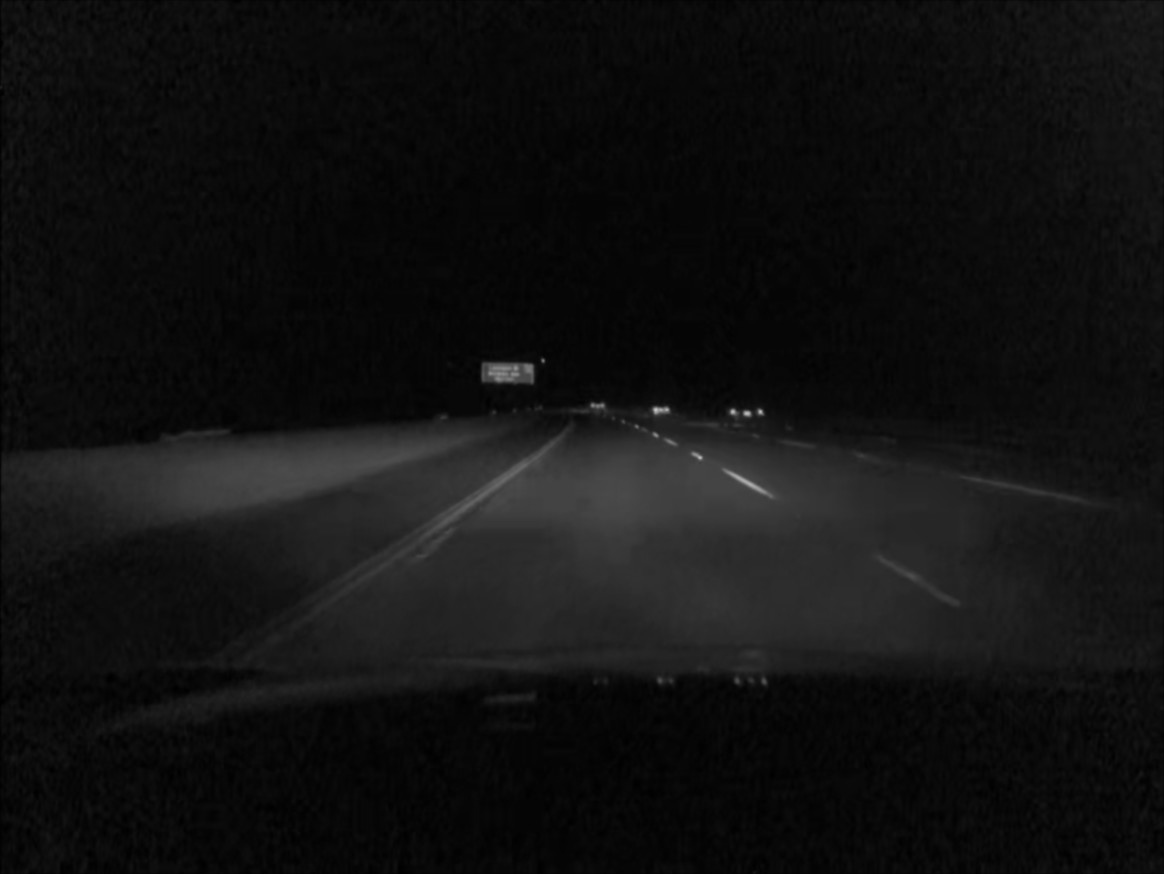
\includegraphics[height=6cm]{result_img/img1_q1.png}
%   \caption{Image 1 : Gaussian Filter}
%   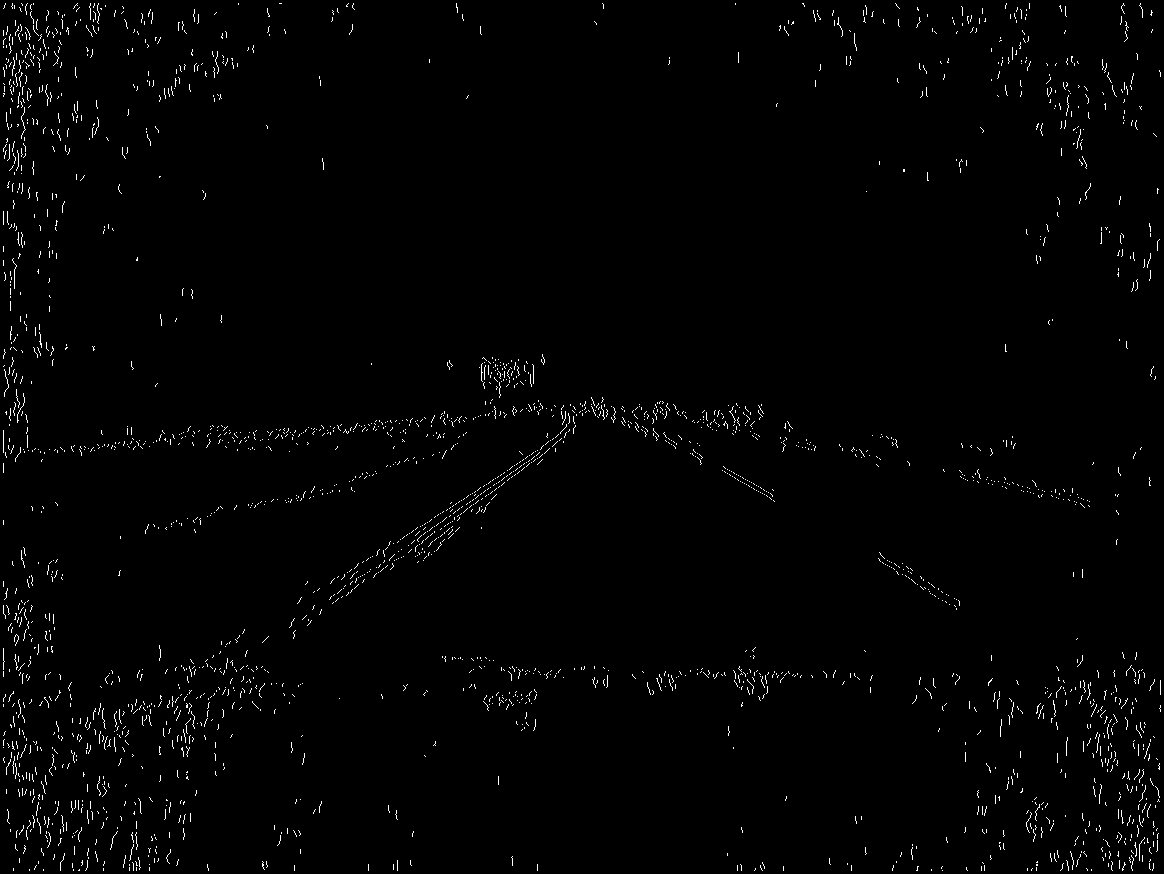
\includegraphics[height=6cm]{result_img/img1_q2.png}
%   \caption{Image 1 : Canny Filter}
%   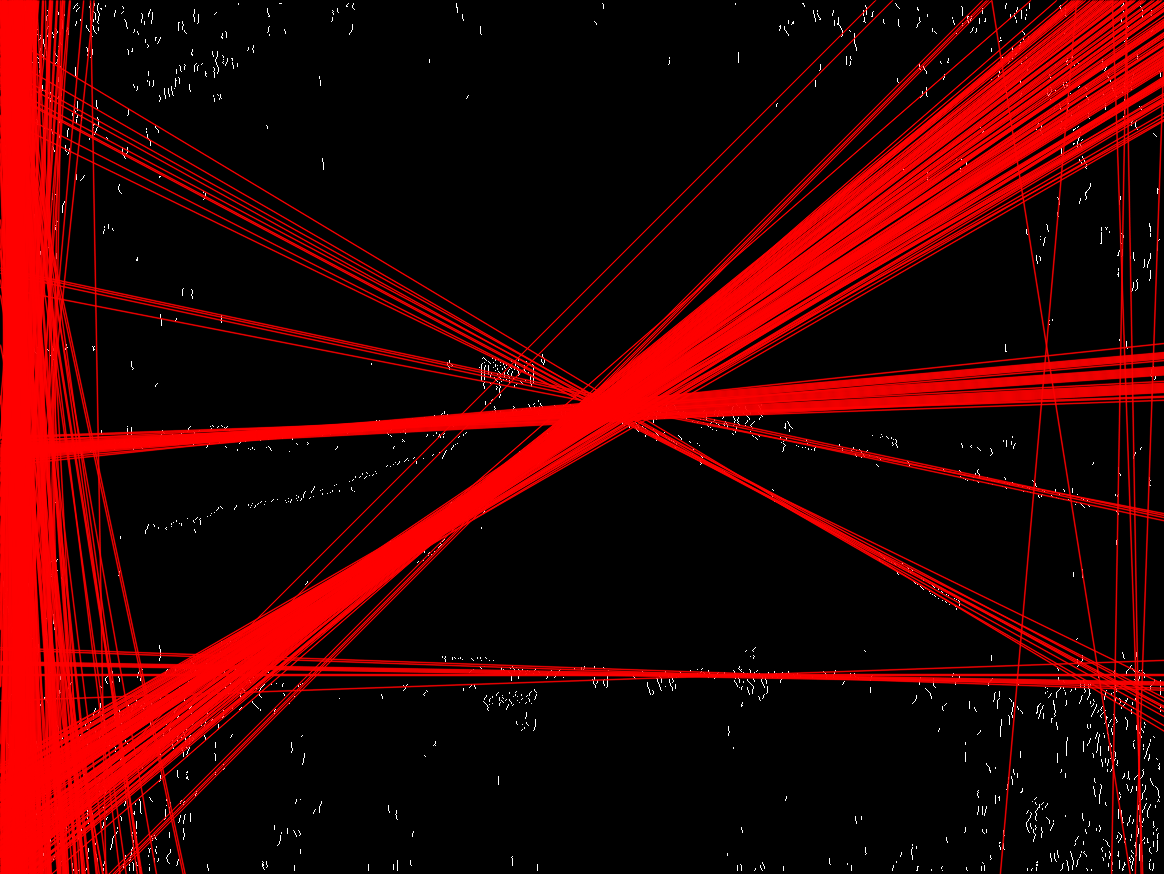
\includegraphics[height=6cm]{result_img/img1_q3.png}
%   \caption{Image 1 : Hough Line Detector}
% \end{figure}
% \begin{figure}[!htb]
%   \centering
%   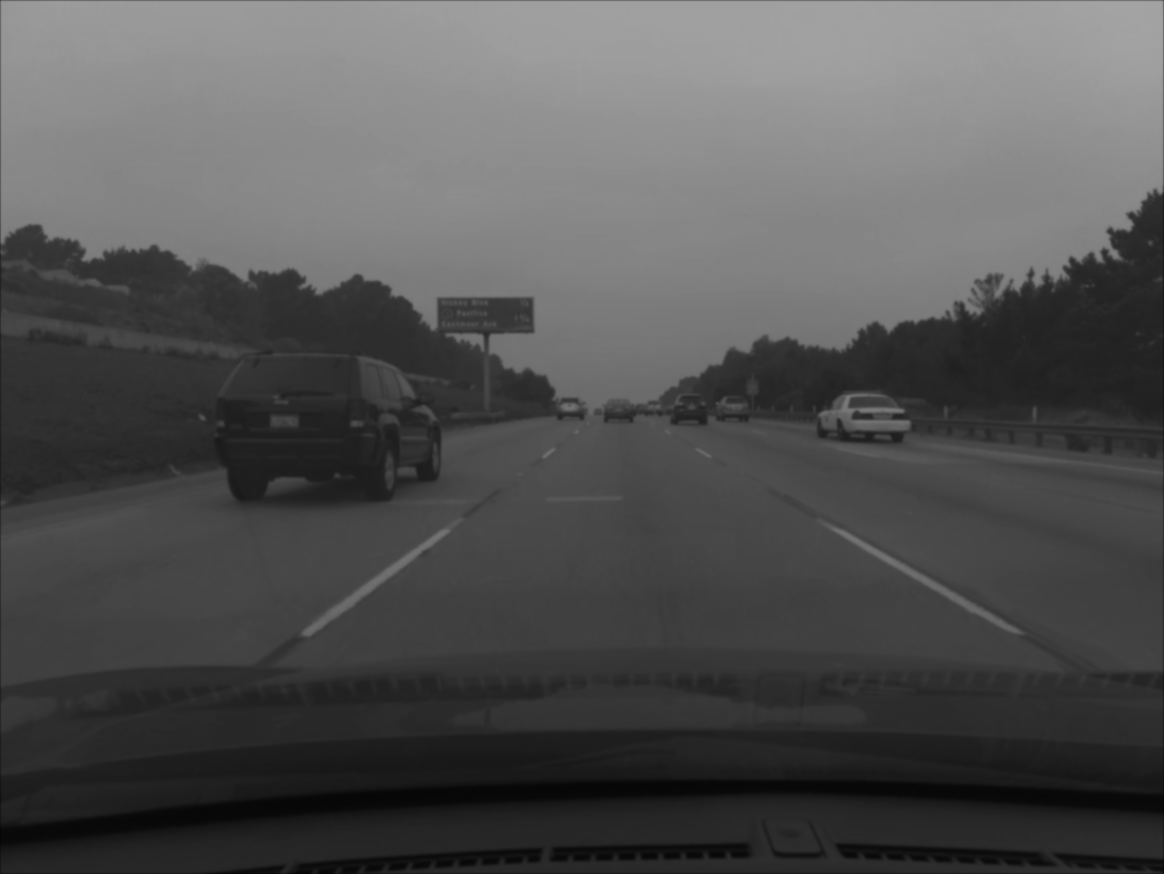
\includegraphics[height=6cm]{result_img/img2_q1.png}
%   \caption{Image 2 : Gaussian Filter}
%   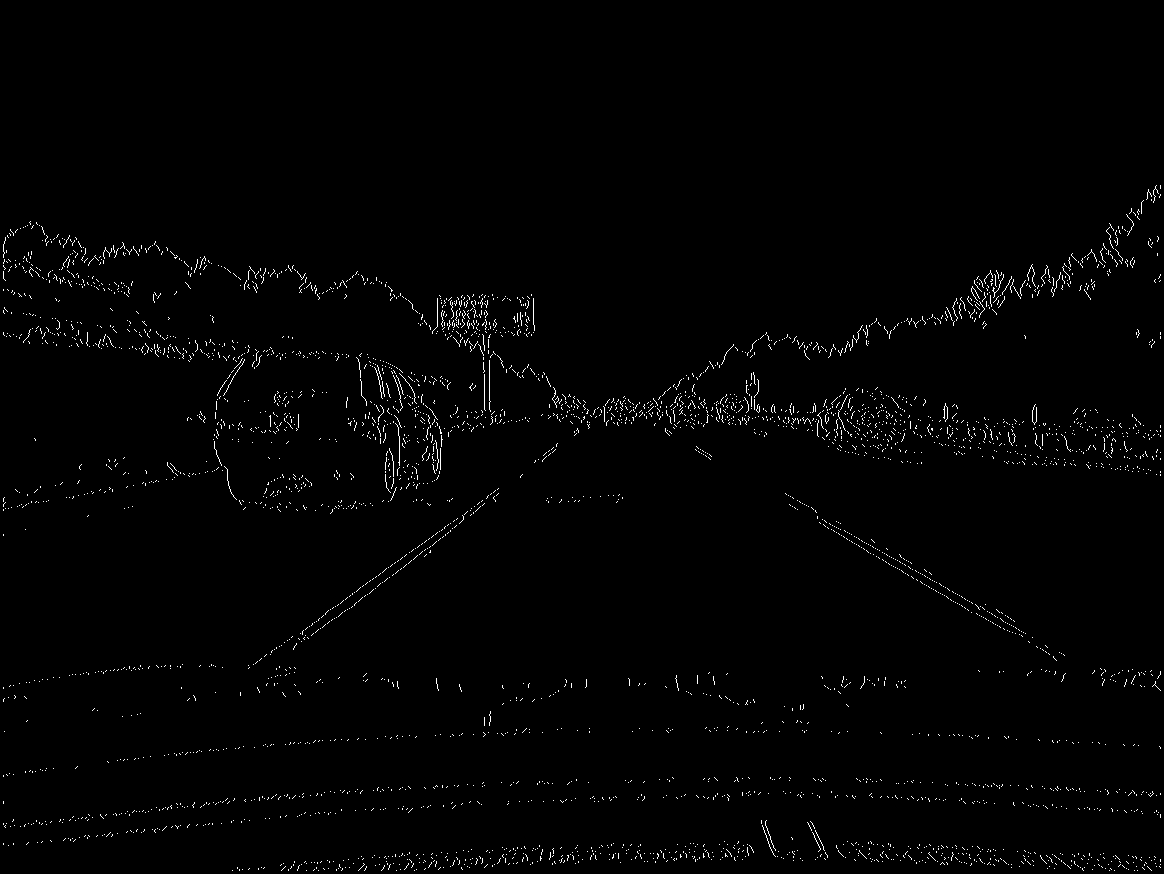
\includegraphics[height=6cm]{result_img/img2_q2.png}
%   \caption{Image 2 : Canny Filter}
%   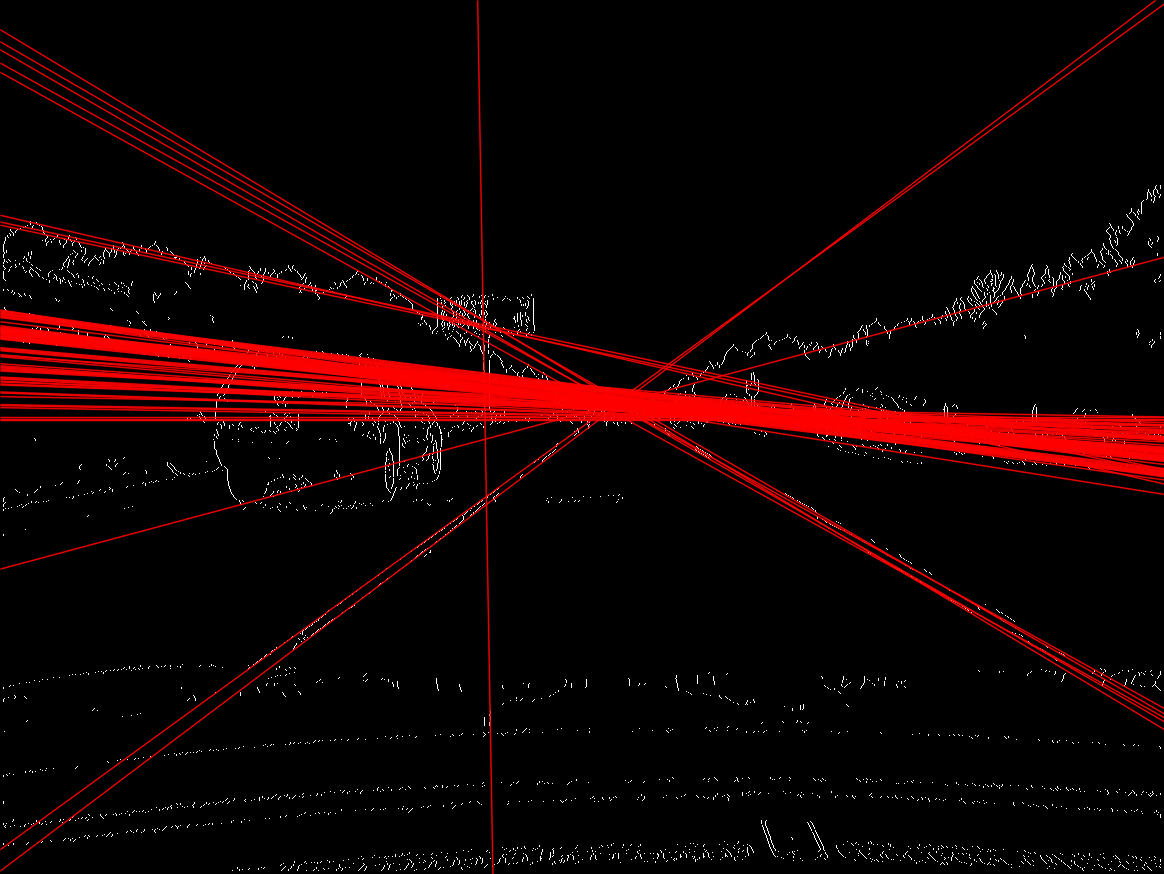
\includegraphics[height=6cm]{result_img/img2_q3.png}
%   \caption{Image 2 : Hough Line Detector}
% \end{figure}
% \begin{figure}[!htb]
%   \centering
%   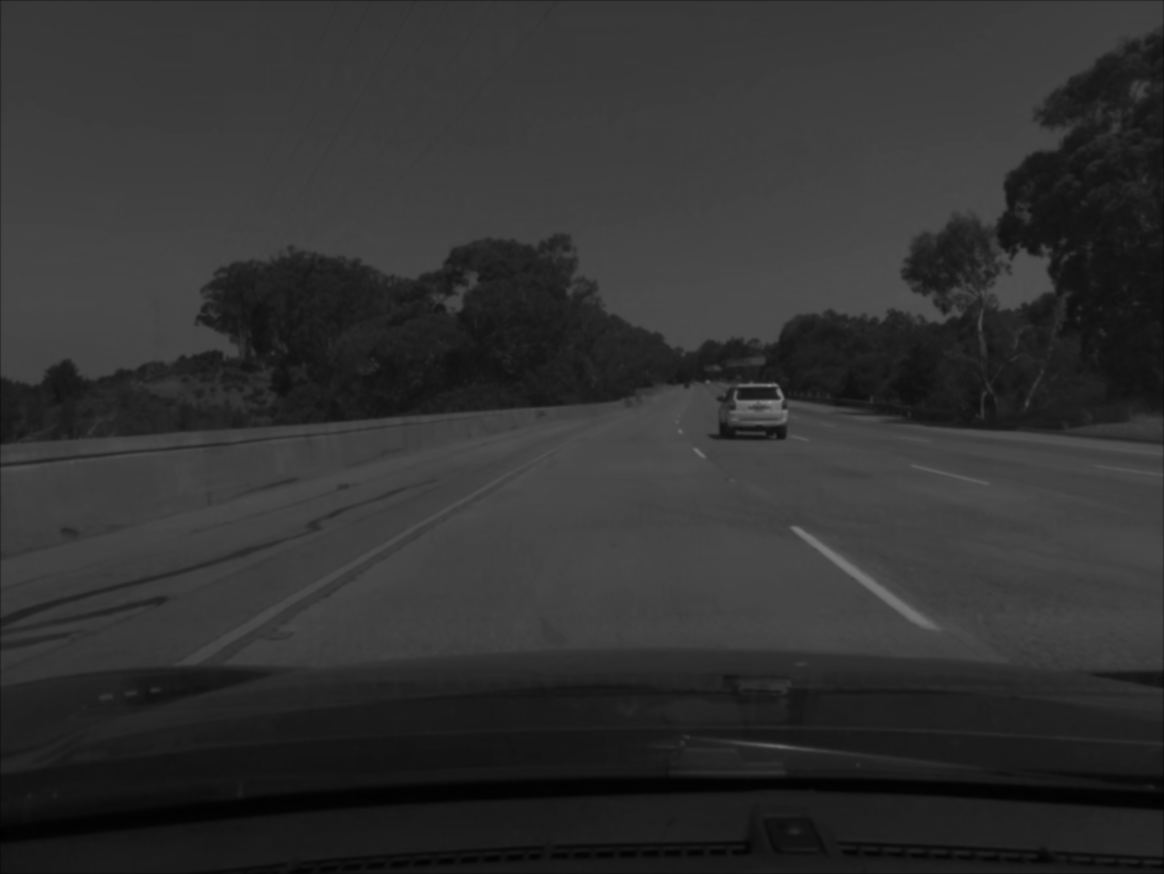
\includegraphics[height=6cm]{result_img/img3_q1.png}
%   \caption{Image 3 : Gaussian Filter}
%   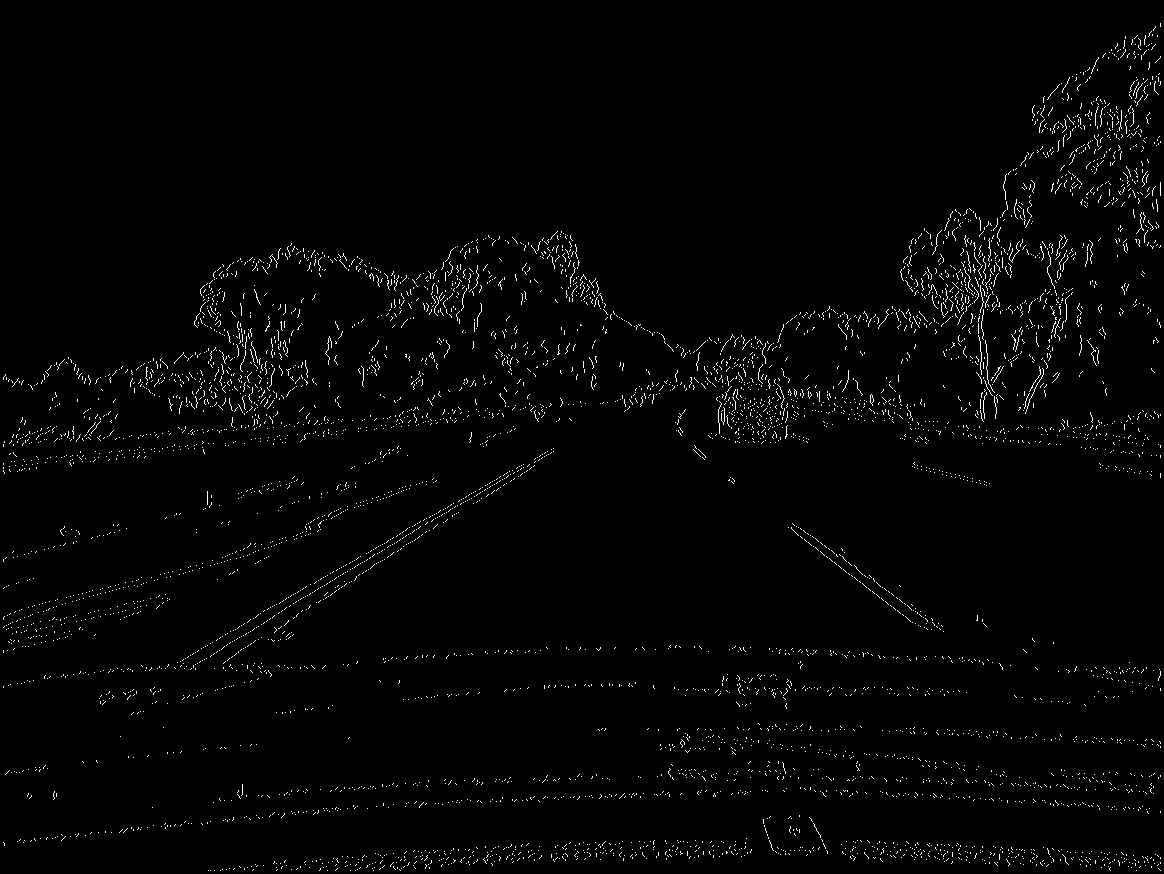
\includegraphics[height=6cm]{result_img/img3_q2.png}
%   \caption{Image 3 : Canny Filter}
%   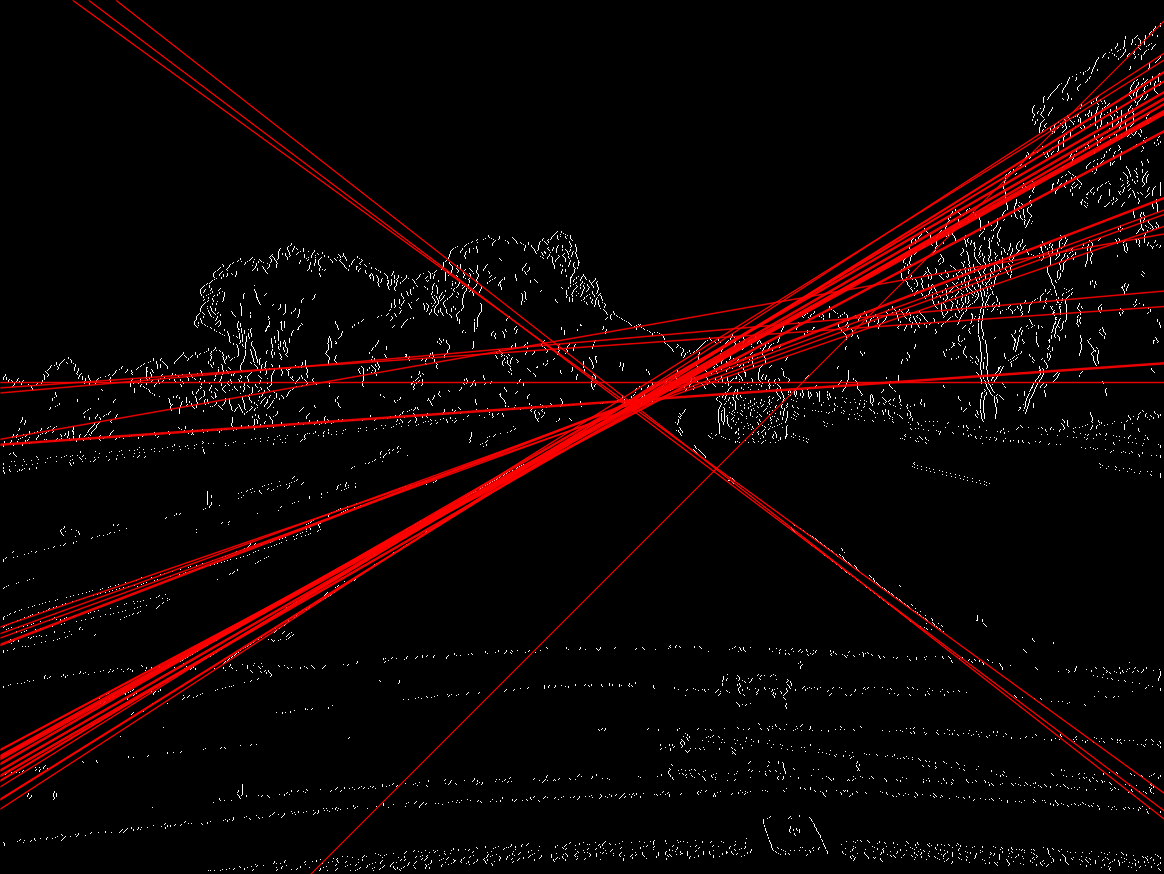
\includegraphics[height=6cm]{result_img/img3_q3.png}
%   \caption{Image 3 : Hough Line Detector}
% \end{figure}
\end{document}
